\documentclass[11pt]{article}

\usepackage{float}
\usepackage{hyperref}
\usepackage{graphicx}
% formatting
\usepackage{fullpage}
\usepackage{verbatim}
\usepackage{moreverb}
\usepackage{minted}
\usepackage{amsmath}
\usepackage{parskip}
\let\verbatiminput=\verbatimtabinput
\def\verbatimtabsize{4\relax}

\begin{document}
\title{EE142 Lab 0.5 Report - VNA Calibration \\
Lab 1 Pre-lab - Passives @ RF}

\author{Vighnesh Iyer \\
Department of Electrical Engineering and Computer Sciences\\
College of Engineering, University of California, Berkeley}
\date{}
\maketitle

\section{VNA Calibration: Testing Cable Phase Stability}

\subsection{Two-Port Technique}
We connect a SMA cable between port 1 and 2. 

Before connecting the cable, the SMA connector's pin depth and dielectric depth are both checked and are within spec. Also, the SMA connector was examined under a stereo microscope and it was cleaned with a cotton swab and alcohol to remove surface contaminants (specks of dirt and metal fragments).

\begin{figure}[H]
	\minipage{0.50\textwidth}
	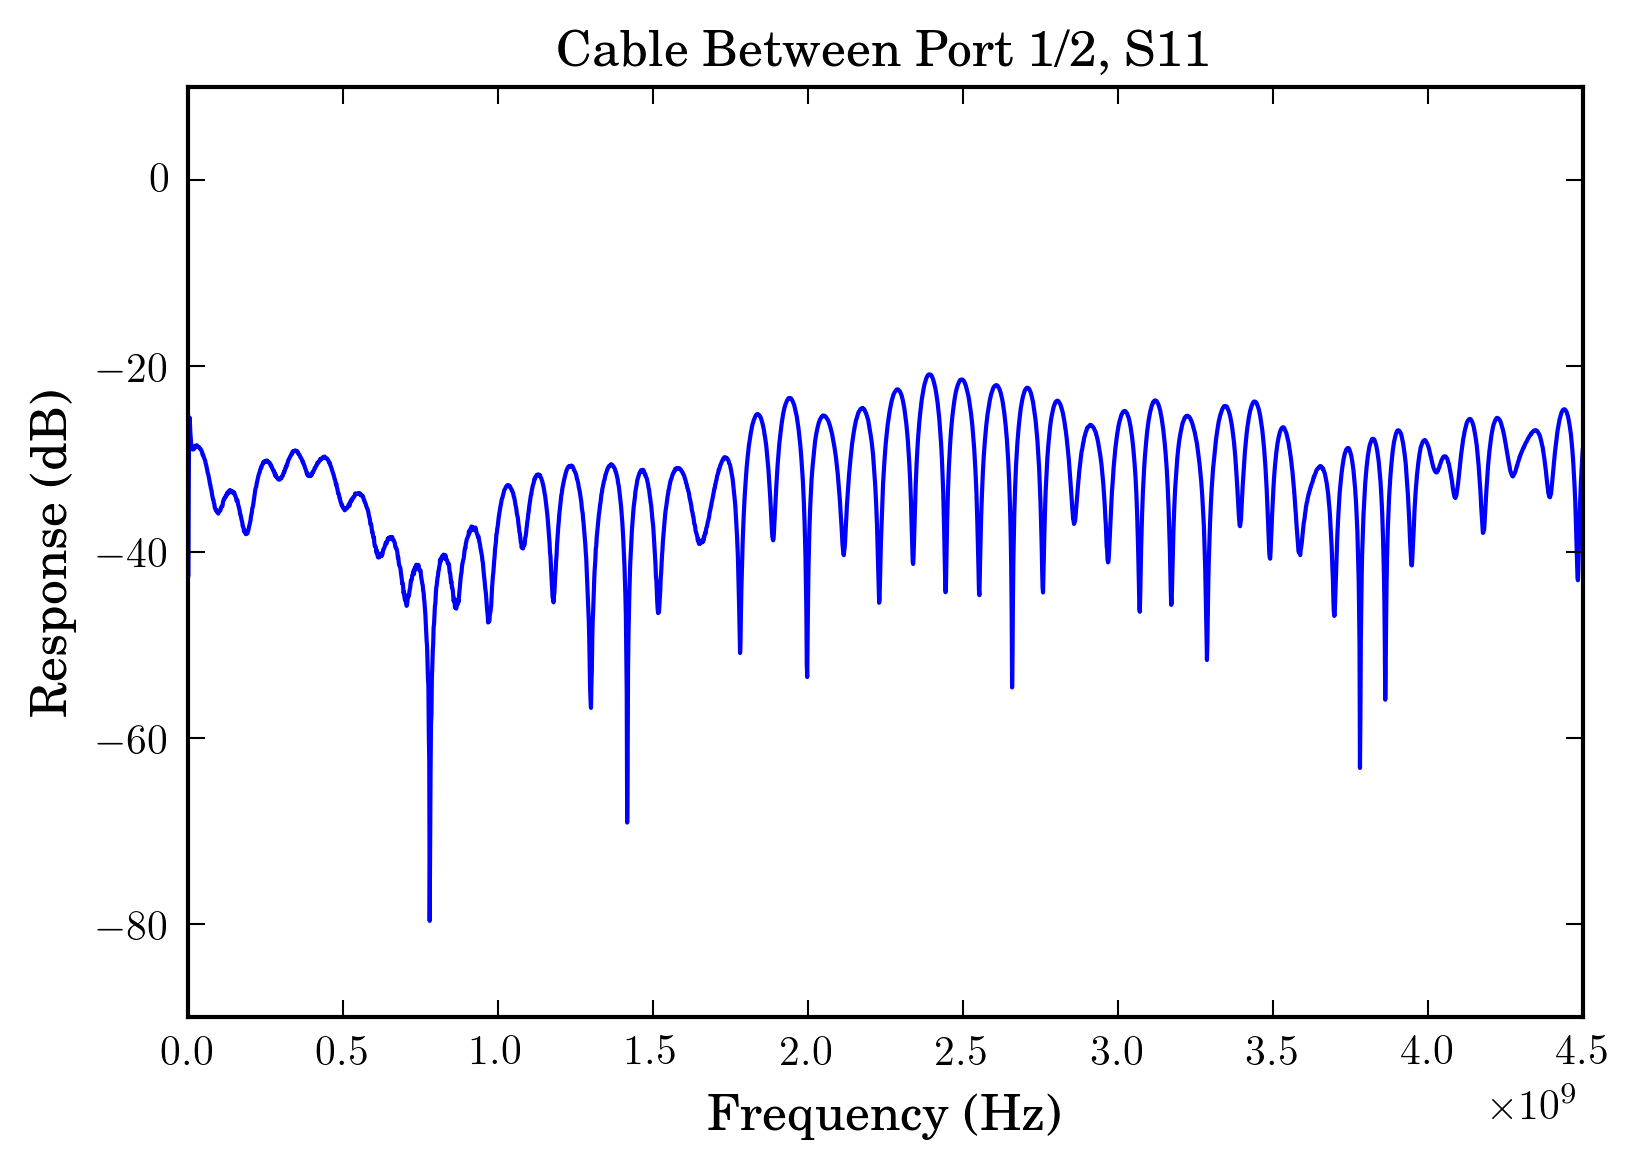
\includegraphics[width=\linewidth]{images/cable_phase_s11.png}
	\endminipage\hfill
	\minipage{0.50\textwidth}
	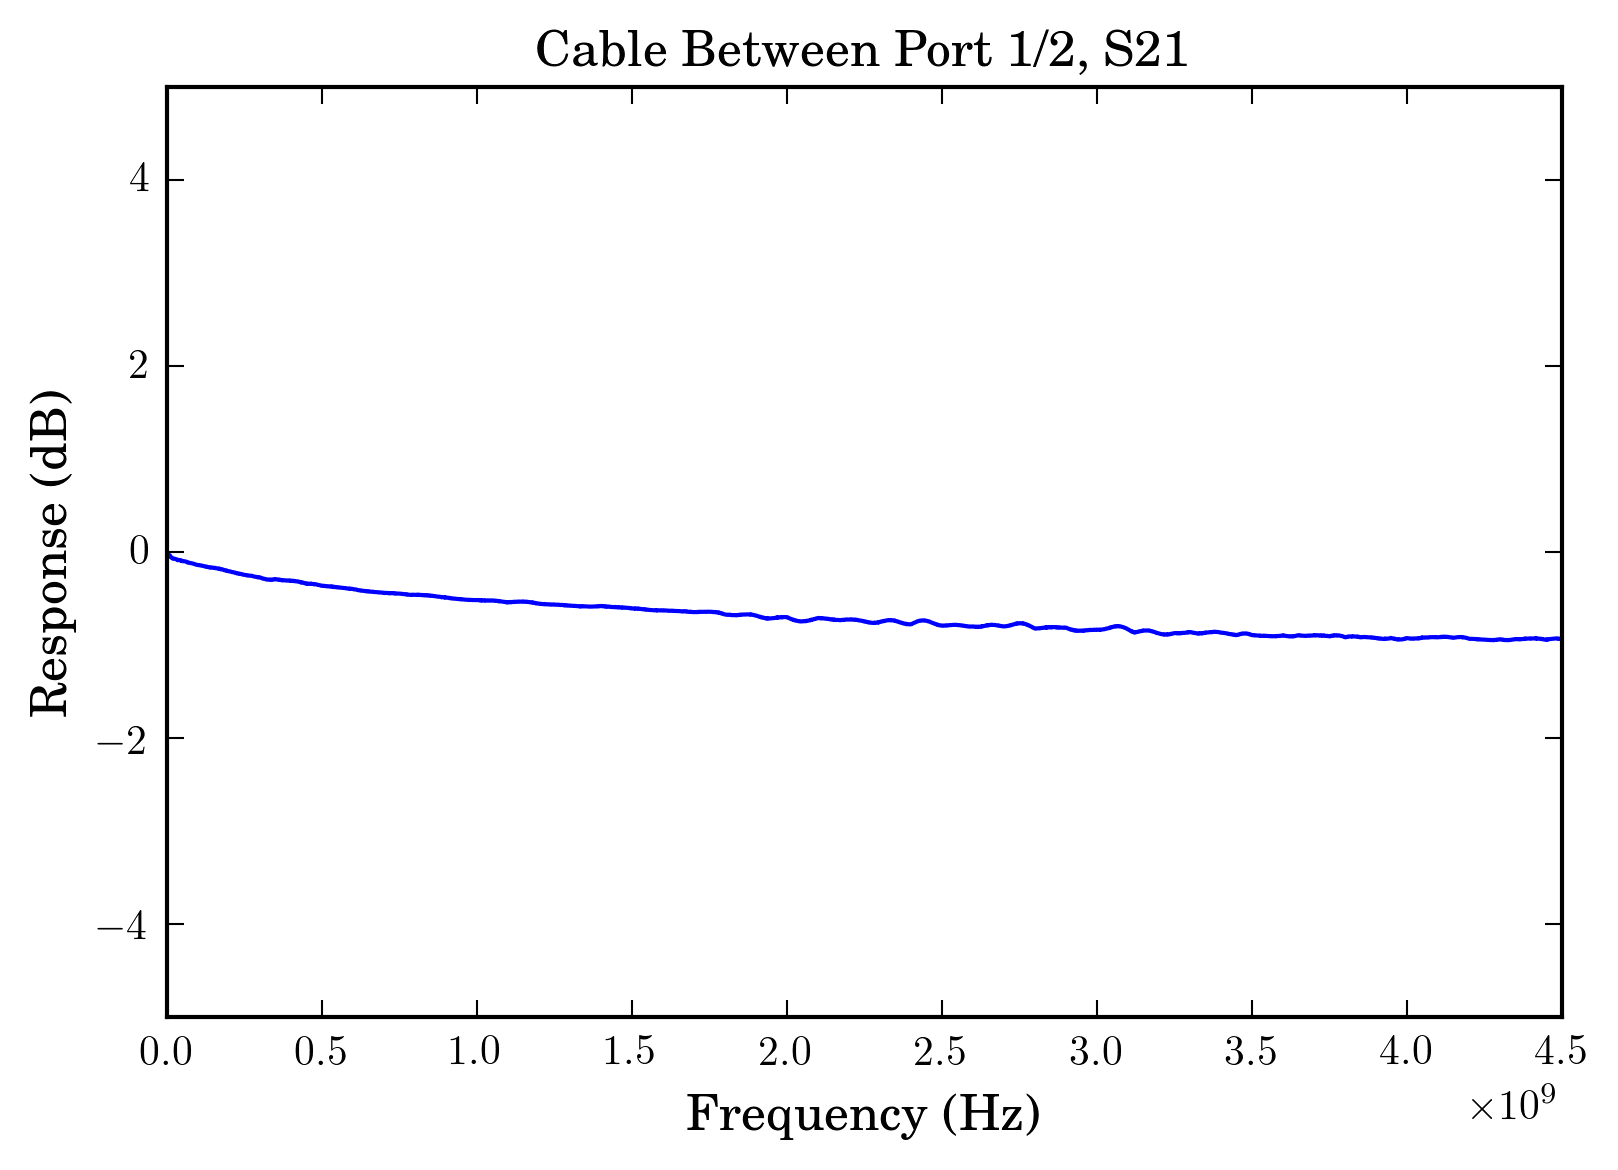
\includegraphics[width=\linewidth]{images/cable_phase_s21.png}
	\endminipage
\end{figure}

When plotting $S_{11}$, we see reflections and re-reflections 20 dB down which show discontinuities in the cable's impedance. When measuring $S_{21}$, we see that almost all the delivered power from port 1 makes its way to port 2 and we only see some drop-off at higher frequencies.


We then look at the phase of $S_{21}$. As expected, the phase wraps around several times for its given length. We then divide the current trace by the last captured trace using the \verb|Data/Memory| function of the NA. Both plots are shown.

\begin{figure}[H]
	\minipage{0.50\textwidth}
	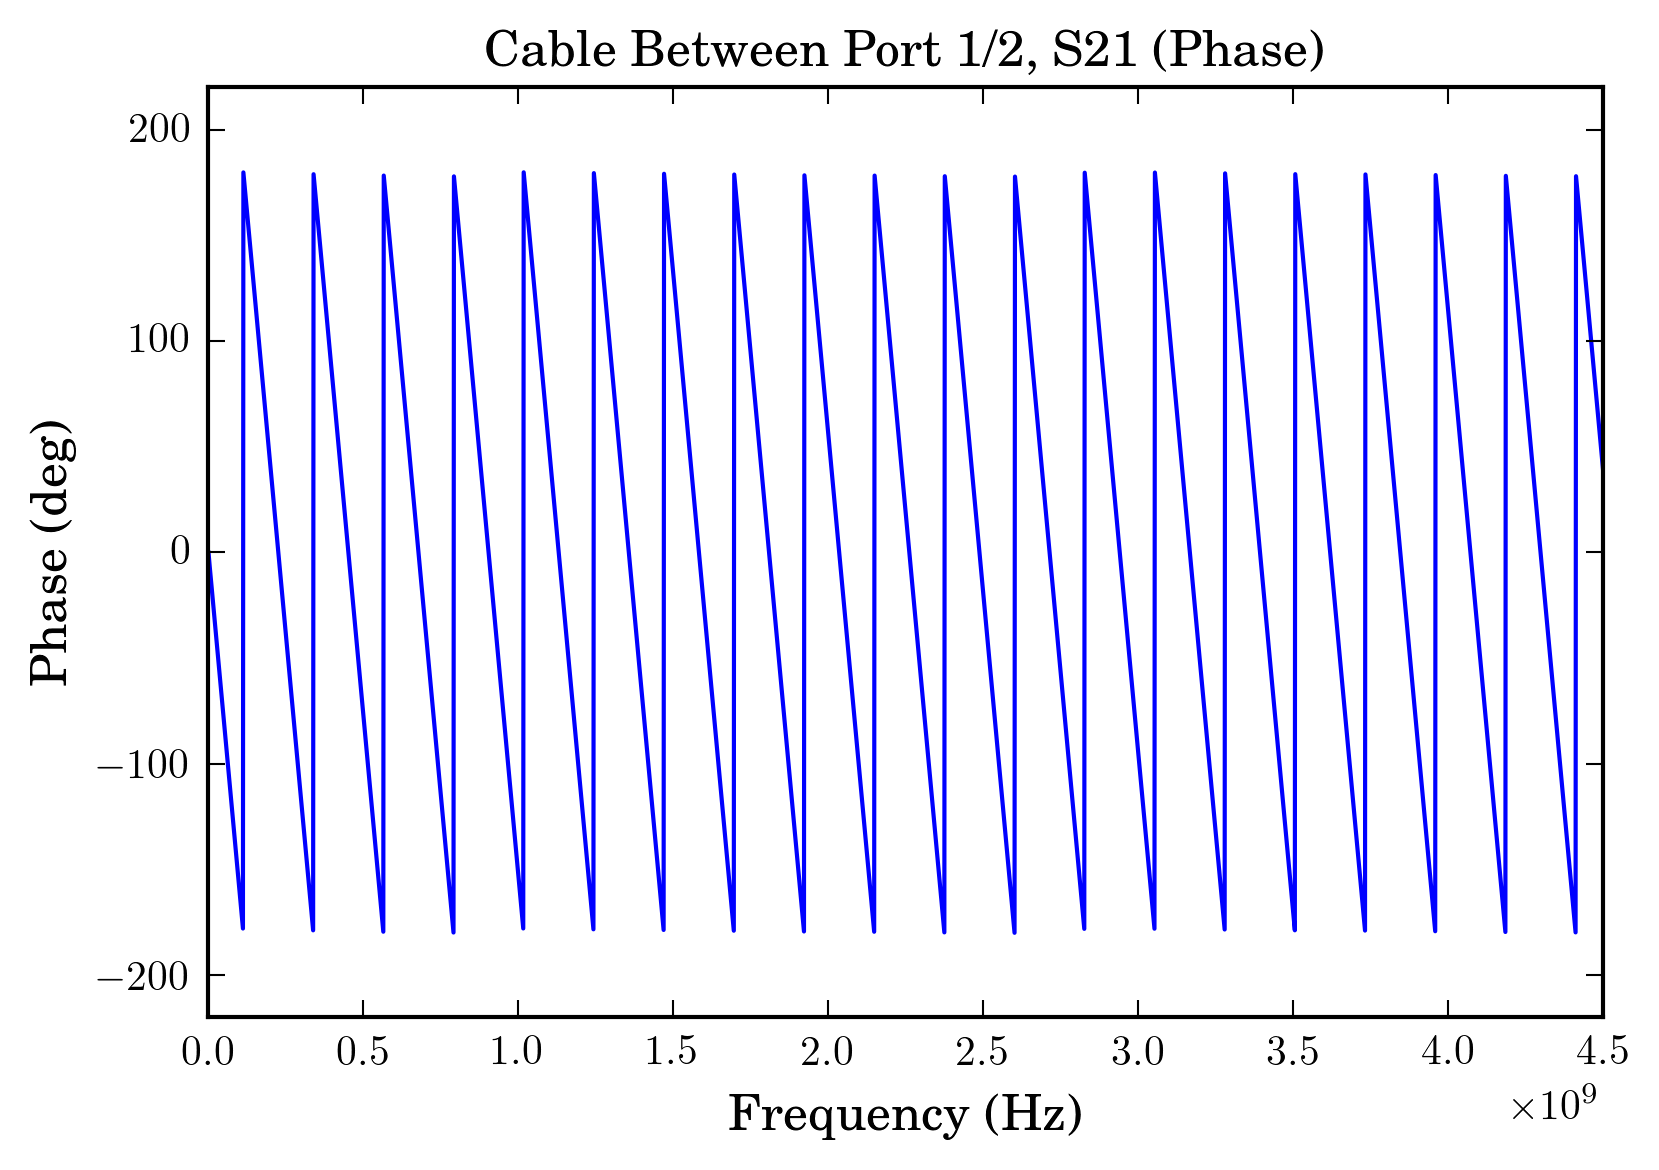
\includegraphics[width=\linewidth]{images/cable_phase_s21_phase.png}
	\endminipage\hfill
	\minipage{0.50\textwidth}
	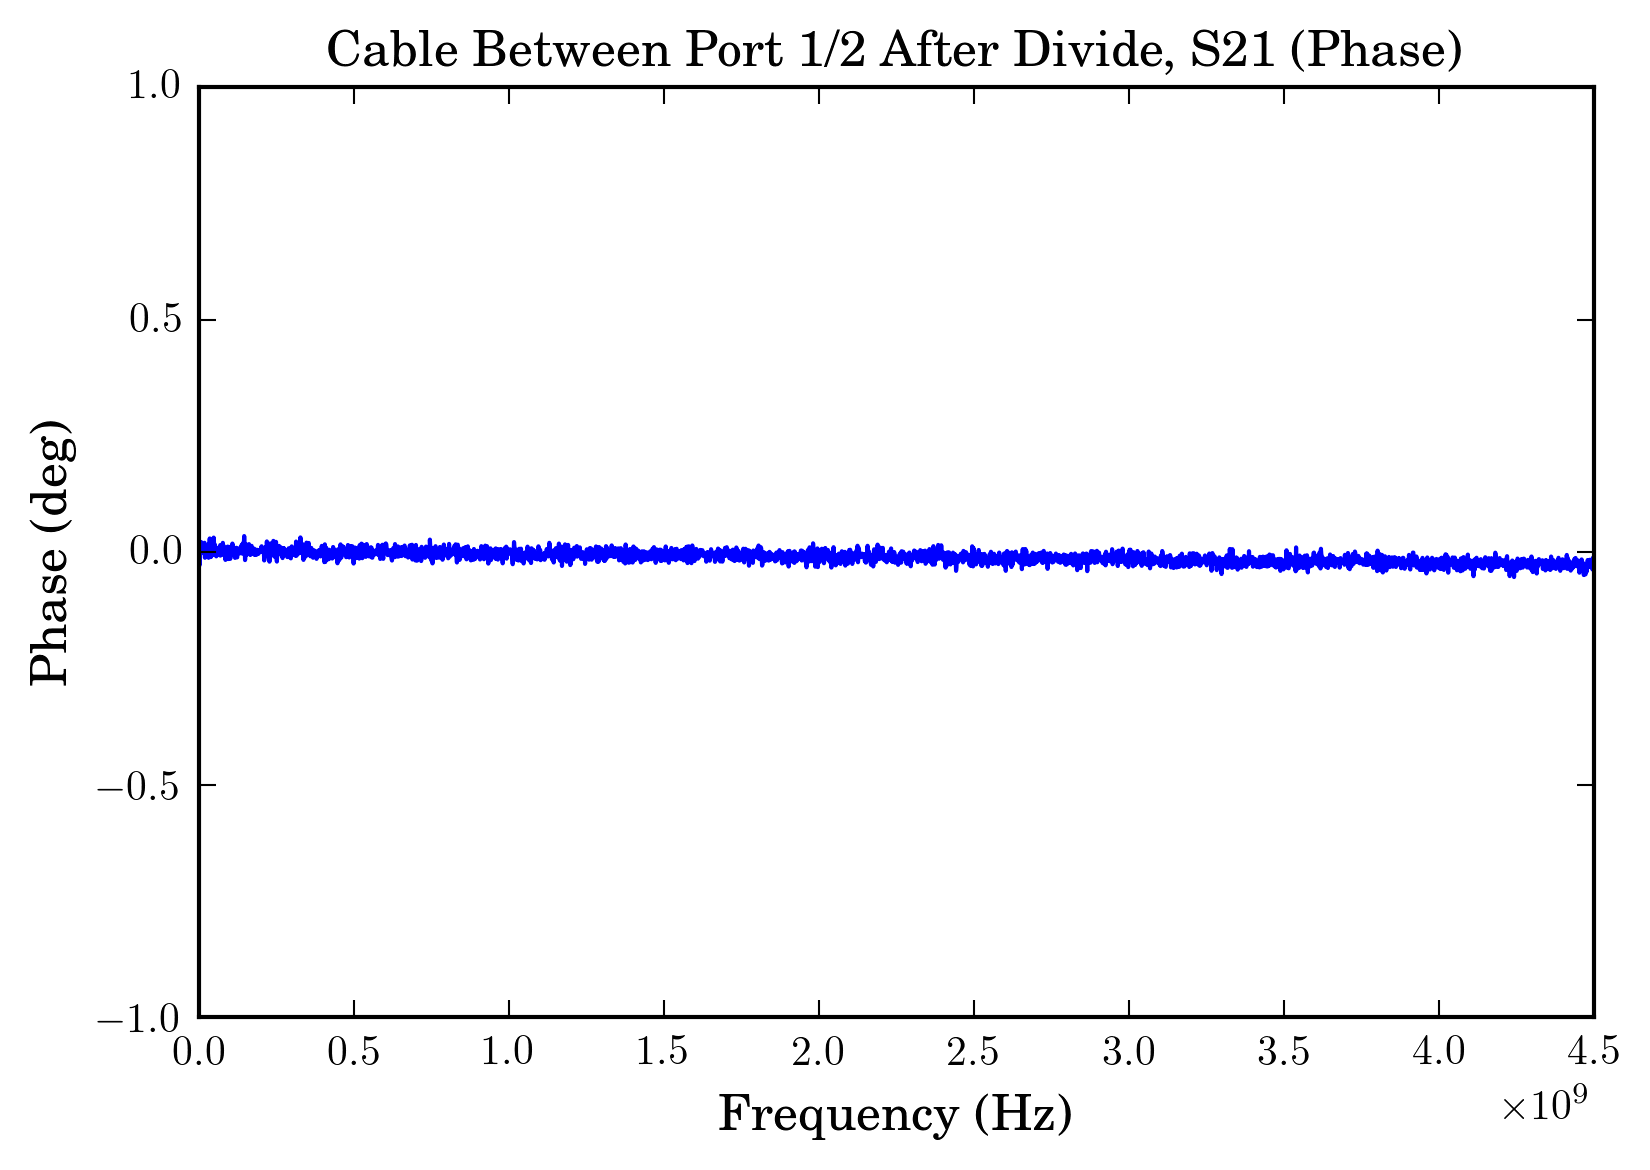
\includegraphics[width=\linewidth]{images/cable_phase_s21_after_data_divide.png}
	\endminipage
\end{figure}

Now, we wiggle and bend the cable several times. The phase of the cable changes due to changes in its electrical length. After some movement, we let the cable sit on the lab bench again until the phase trace settles.

\begin{figure}[H]
	\centering 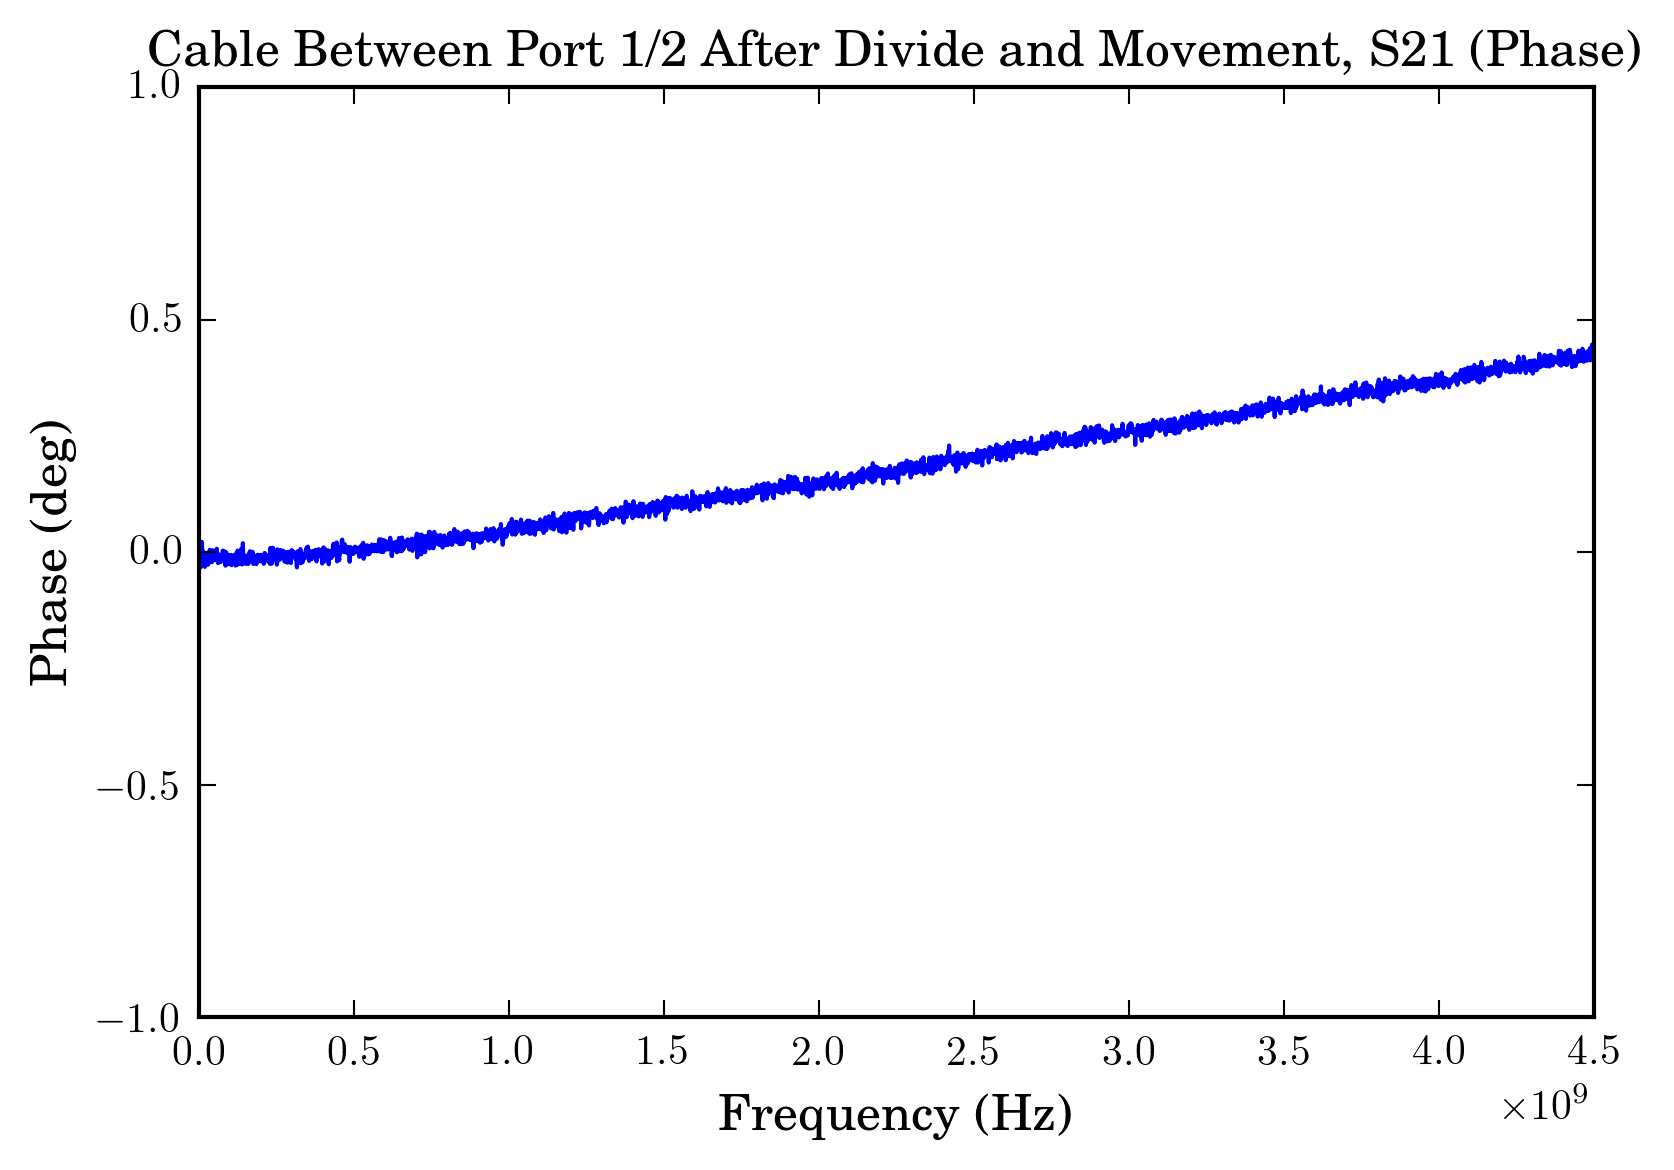
\includegraphics[width=\linewidth-7cm]{images/cable_phase_s21_after_movement.png}
\end{figure}

We see some positive phase on the upper frequencies, but only less than 0.5 degrees. This cable seems to have decent phase stability.

\subsection{One-Port with Cal Standard Technique}

We connect one end of a SMA cable to port 1 and the other end to a open calibration standard. The display is set to Log-Mag $S_{11}$.

The cable is placed down and we use the \verb|Data->Mem| = \verb|Data-Mem| to subtract out the last captured trace from the current trace. This pushes the Log-Mag trace to around -60 dB, but I expected the trace to plunge further down to -80 dB closer to the noise floor of the instrument.

\begin{figure}[H]
	\centering 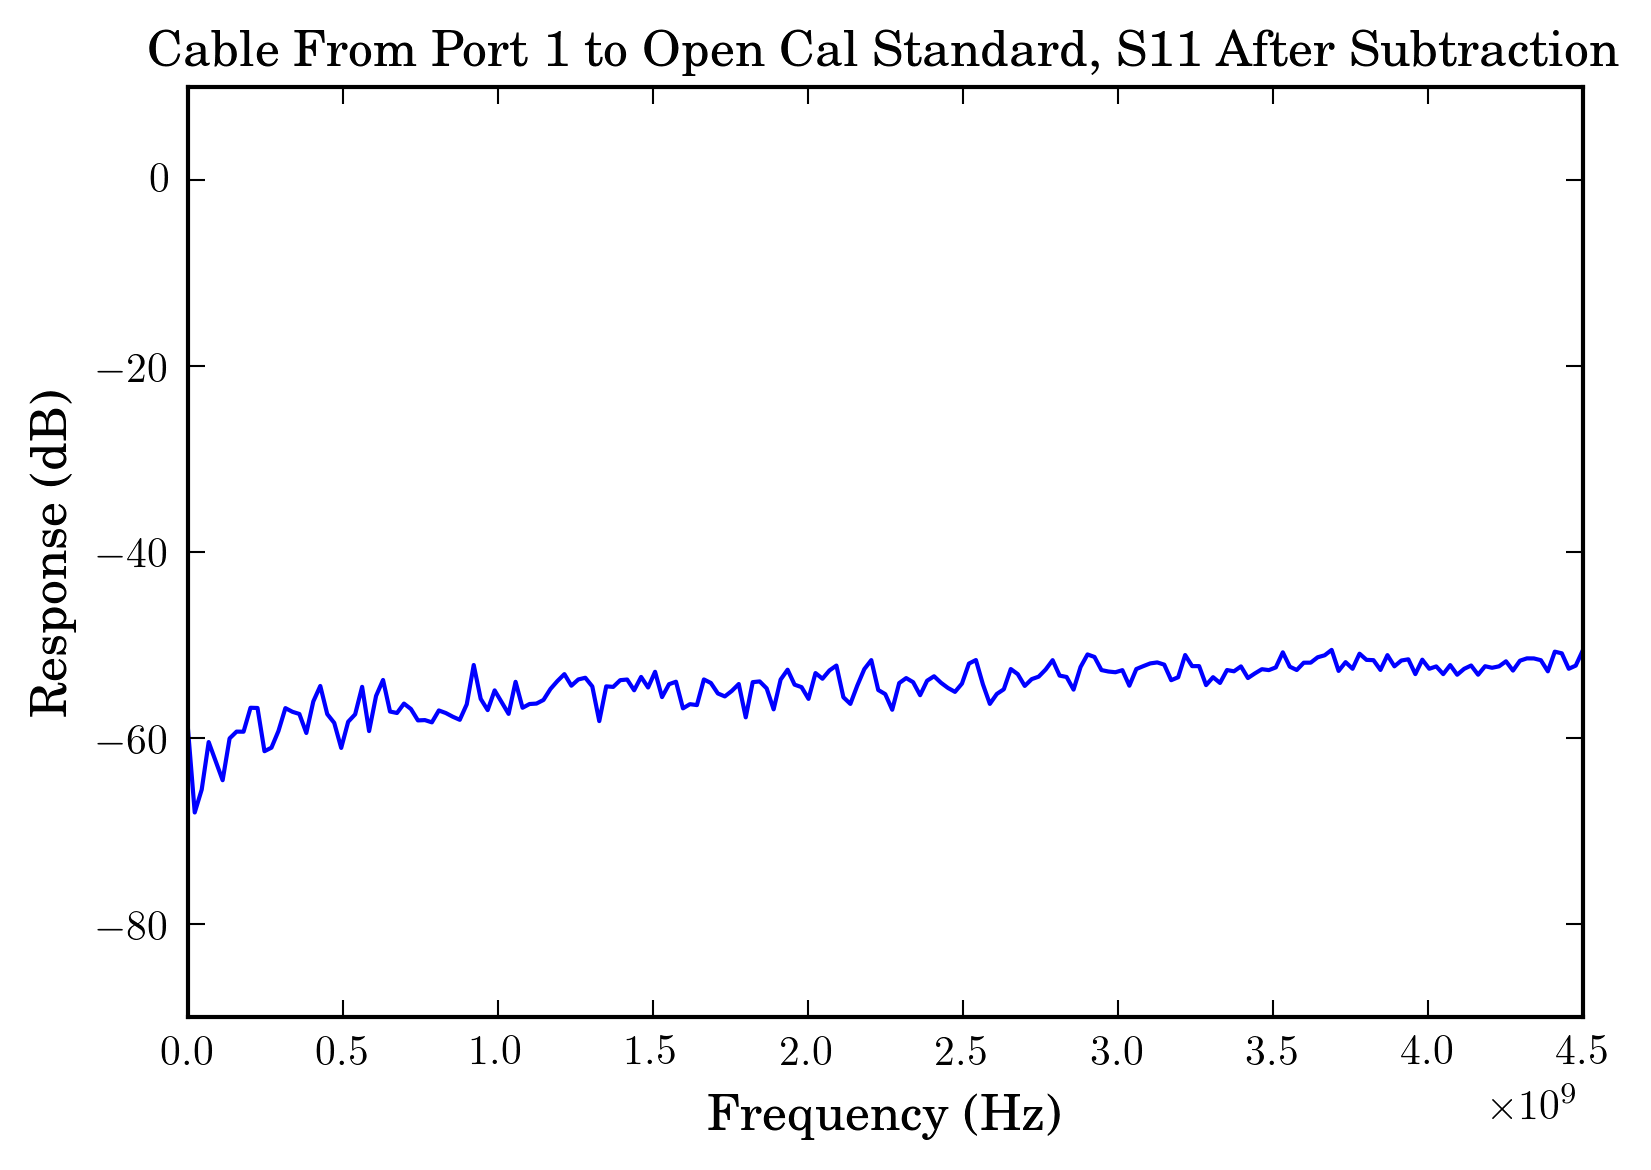
\includegraphics[width=\linewidth-6cm]{images/one_port_s11_open_cal.png}
\end{figure}

Finally, the cable is moved around and flexed for 10 seconds, and the cable is placed down on the lab bench again. The trace is allowed to settle down.

\begin{figure}[H]
	\centering 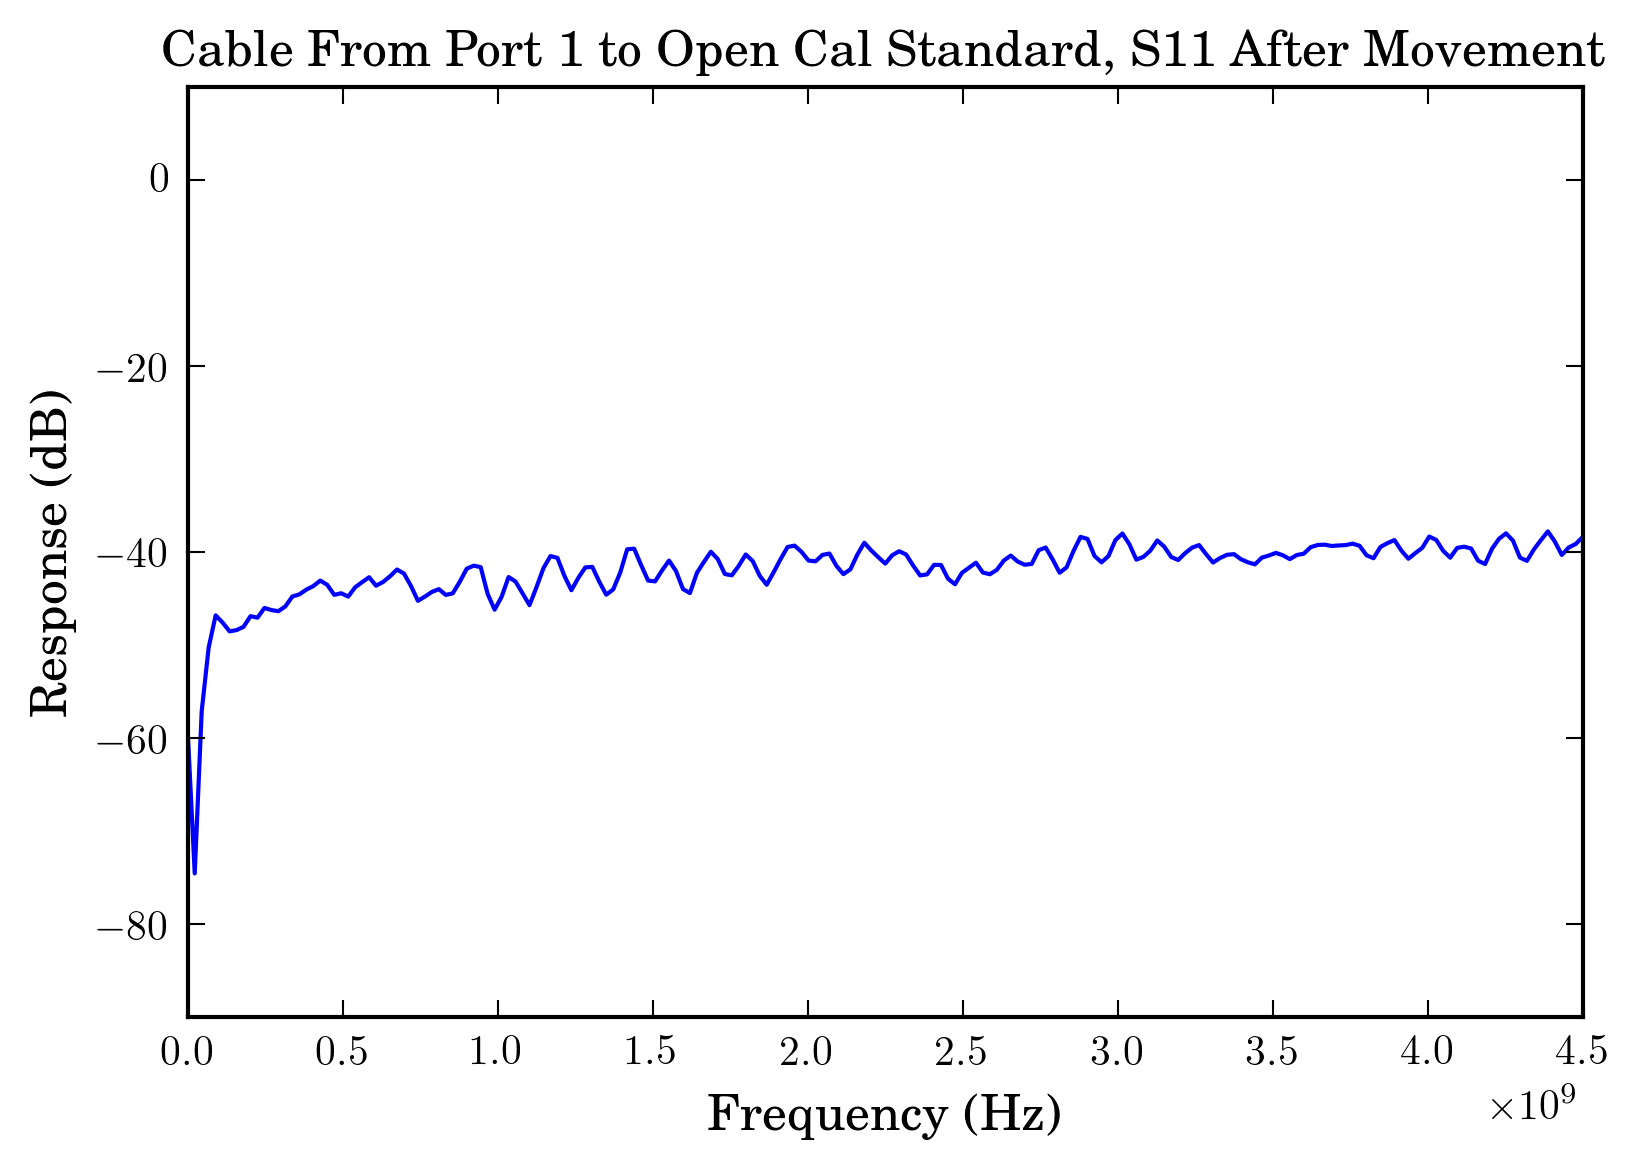
\includegraphics[width=\linewidth-6cm]{images/one_port_s11_open_cal_after_movement.png}
\end{figure}

The trace should have moved from its -80 dB state upwards as the cable's electrical length/phase has been slightly changed due to the movement. A very good cable moves to around -50 dB, while a decent cable moves to around -40 dB. A poor cable will move up to -30 dB or higher.

We can see that our chosen cable is of mid-range quality and has enough phase stability to perform reliable measurements.

\section{VNA Calibration: Calibration using E-Cal}

I performed a one-port calibration using the SOL standards first, but I found that they gave inconsistent results and didn't give a good cal when testing other standards.

I decided to then try the E-Cal, which was easy to set up to calibrate the VNA, with the same set of cables I tested earlier. I performed a full two-port cal.

Here is a Smith chart and $S_{11}$ trace of a open standard directly connected to port 1 (no cable) before E-Cal calibration.

\begin{figure}[H]
	\centering 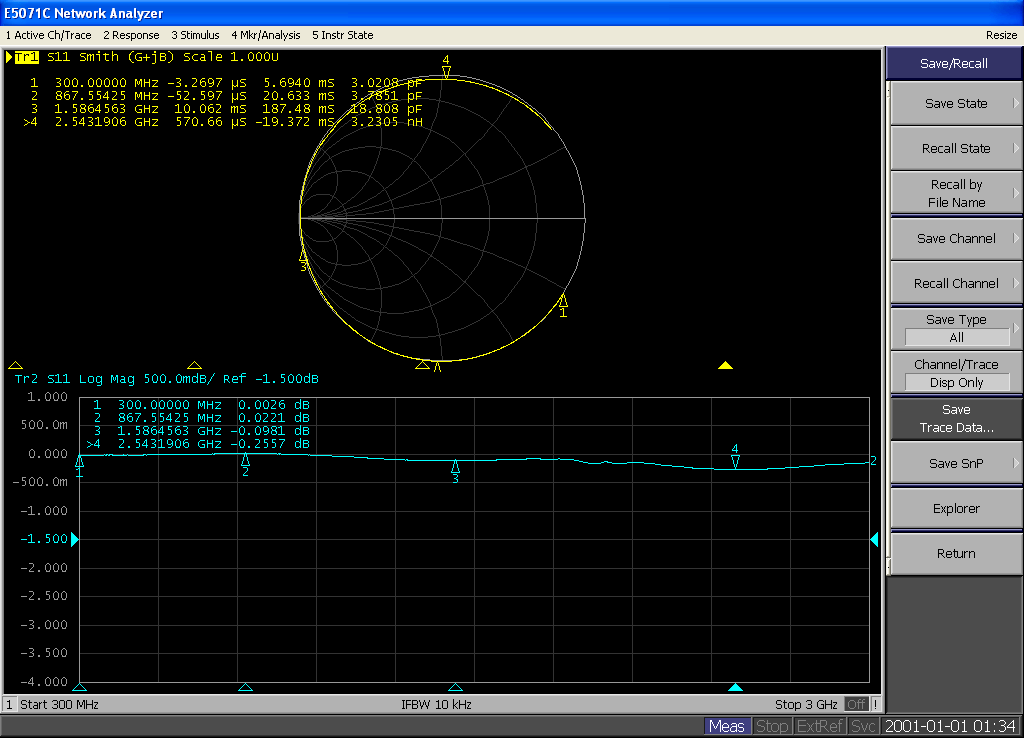
\includegraphics[width=\linewidth-6cm]{images/S11_OPEN_STD_BEFORE_CAL.PNG}
\end{figure}

We can see that the electrical delay isn't compensated for and the open doesn't look perfect.

\section{VNA Calibration: Verifying Calibration With Cal Standards}
After E-Cal calibration with the set of cables I used earlier, I tried connecting an open standard to the end of the cable to check the calibration quality.

\begin{figure}[H]
	\centering 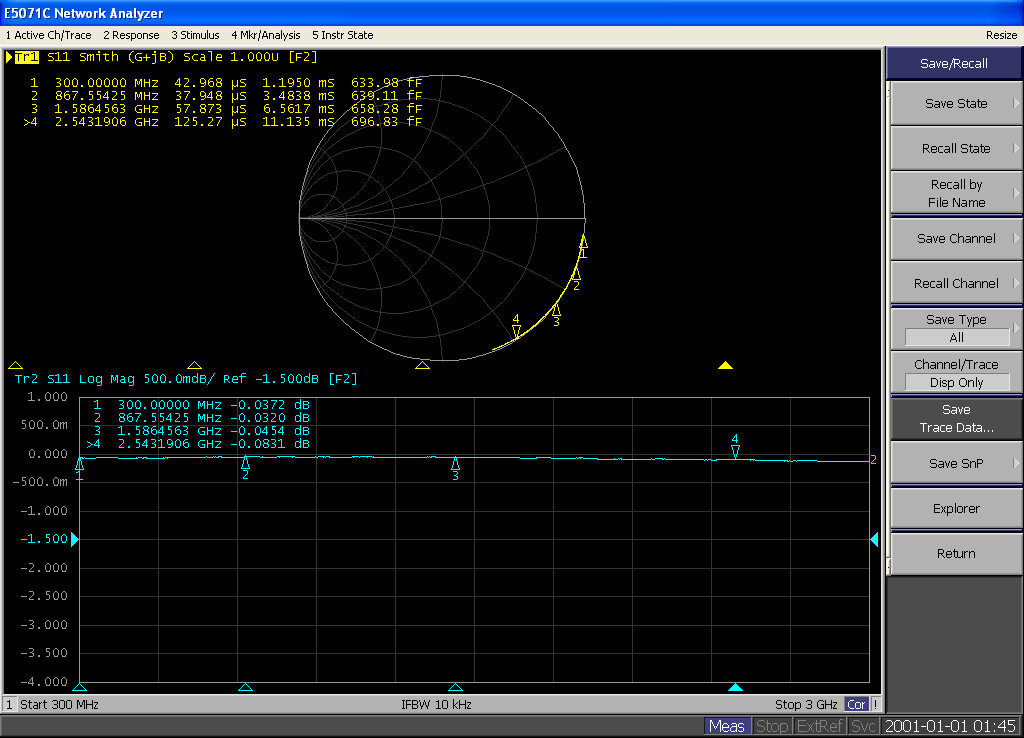
\includegraphics[width=\linewidth-6cm]{images/S11_OPEN_STD_AFTER_CAL.PNG}
\end{figure}

This looks a lot better, and the only issue is the electrical delay of the open standard isn't factored into the measurement. Otherwise, it looks nearly perfect.

Comparing it to the reference from the Calibration powerpoint:

\begin{figure}[H]
	\centering 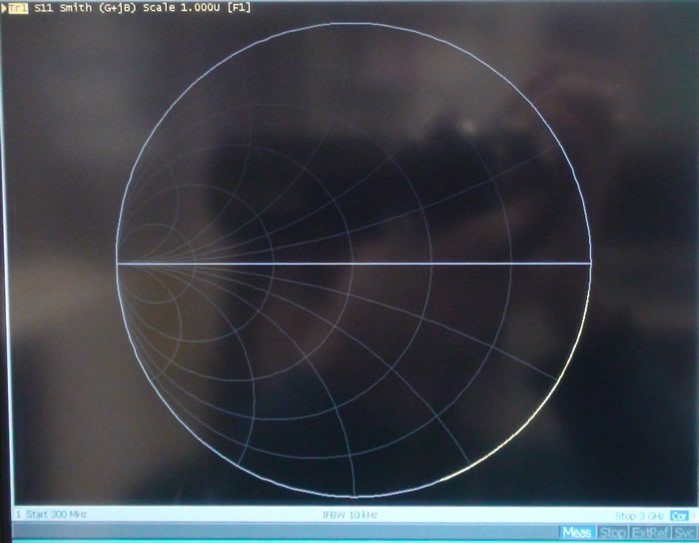
\includegraphics[width=\linewidth-6cm]{images/S11_OPEN_STD_REFERENCE.JPG}
\end{figure}

We can see that it is a very close match before accounting for offset delay and the cable I used not being held perfectly still.


\section{VNA Calibration: Questions}

\begin{enumerate}
	\item Why do we use a torque wrench when making connections?
	
	A torque wrench will mate two connectors such that the impedance mismatch between them is minimized from the connector construction.
	
	\item Why should you never rotate the cal standard when you connect it?
	
	The cal standard's connector contains several fragile fingers that can be damaged by rotating a pin inside of them.
	
	\item How can an SMA cable connector damage a cal standard?
	
	If the SMA cable's pin sticks out more than spec, it can damage the fingers of the cal standard.
	
	\item What is the difference between a 3.5mm connector and an SMA connector?
	
	A 3.5mm connector uses air dielectric versus plastic for SMA and is more fragile. The connectors are compatible however when mated.
	
	\item Where is their reference plane?
	
	The reference plane is at the base of the dielectric for male and female connectors. 
	
	\item Why is it recommended to remove the rubber gaskets from N and SMA connectors?
	
	The rubber gaskets can cause connection issues as they are intended for outdoor use.
	
	\item Why is it a bad idea to use a cal standard as a load for your amplifier?
	
	A cal standard isn't designed to dissipate power and could have its properties changed if subjected to too much power.
	
	\item Why should you turn the power down on the network analyzer when you hook up an amplifier?
	
	The NA's ports can handle at most +26 dBm of power; an amplifier could easily deliver more power than allowable if it's fed too much power at it's input.	
\end{enumerate}

\section{Lab 1 Prelab}

\subsection{Inductor Analysis}
We use the lumped inductor model in Figure 4 of the lab spec:

\begin{figure}[H]
	\centering 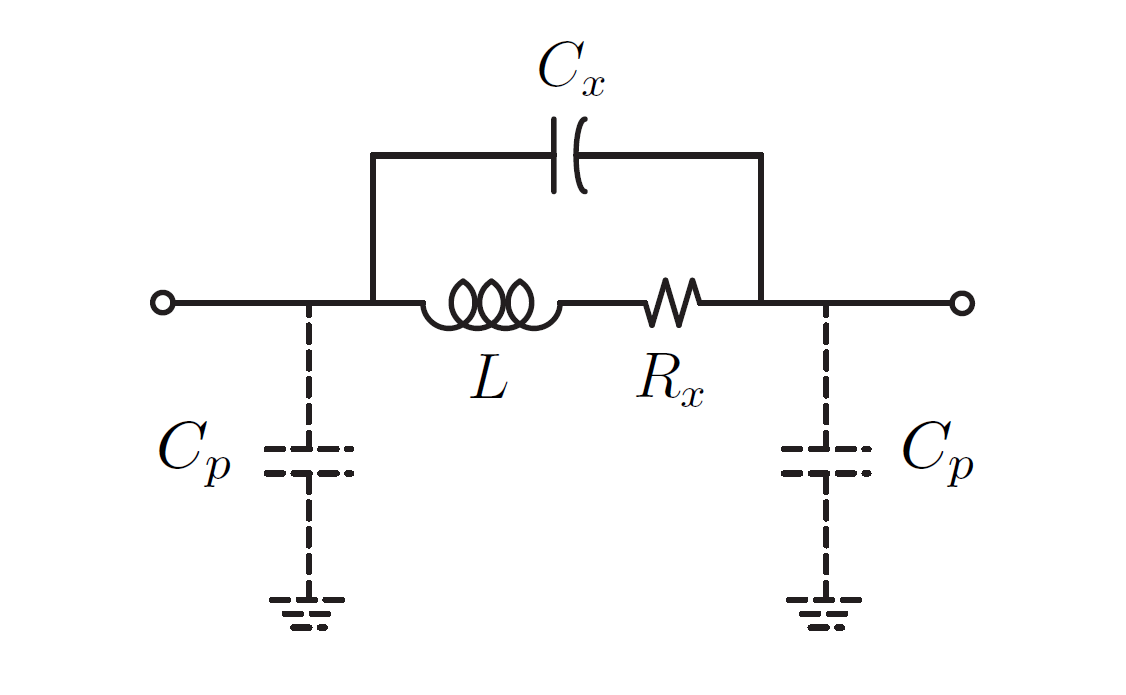
\includegraphics[width=\textwidth-8cm]{images/lumped_inductor_model.png}
\end{figure}

The component values are: $L = 5$ nH, $R_{x} = 1.15\Omega$, $C_{p} = 400$ fF, $C_{x} = 10$ fF.

\subsubsection{Impedance and Inductance Plots}

\begin{figure}[H]
	\centering 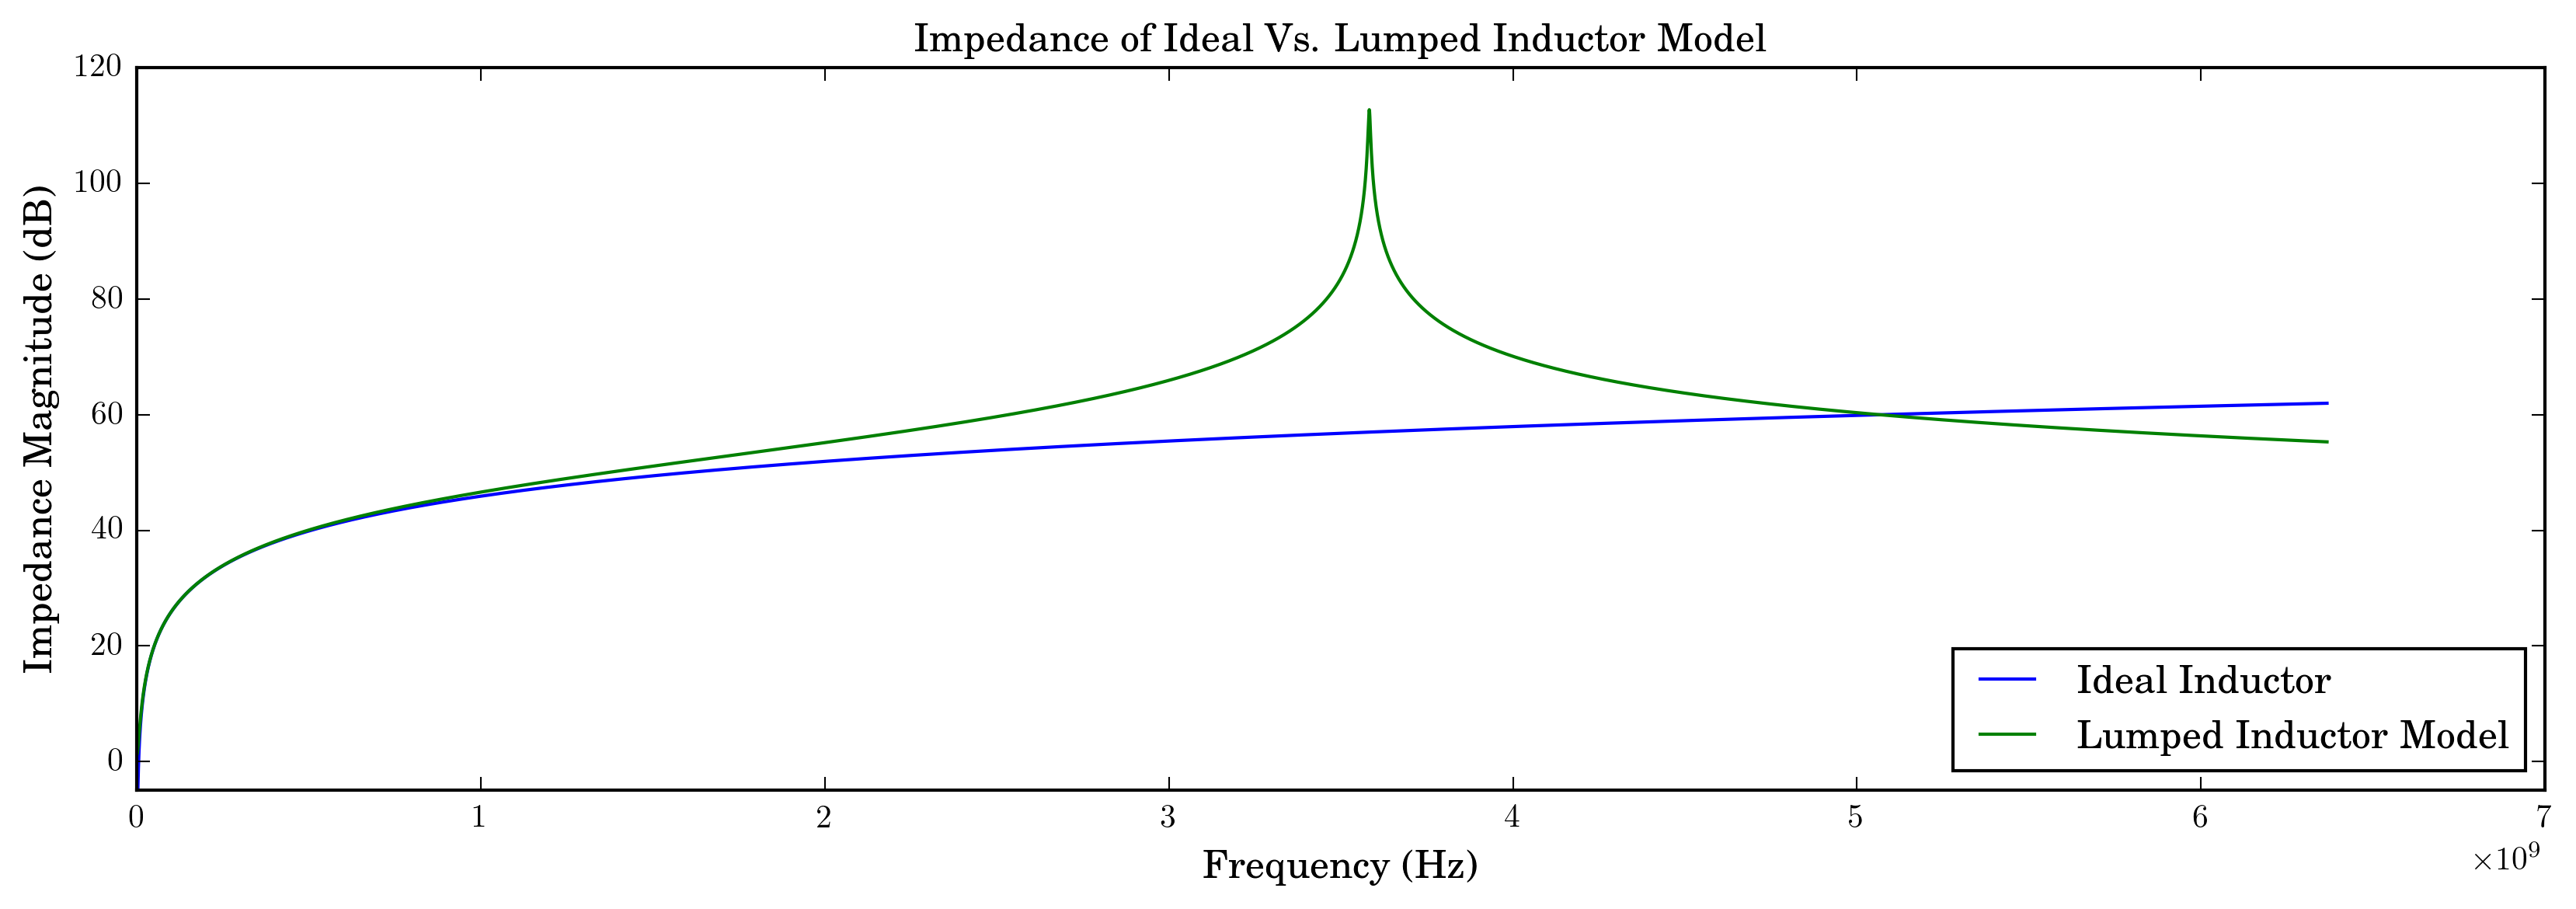
\includegraphics[width=\textwidth]{images/inductor_impedance.png}
\end{figure}
\begin{figure}[H]
	\centering 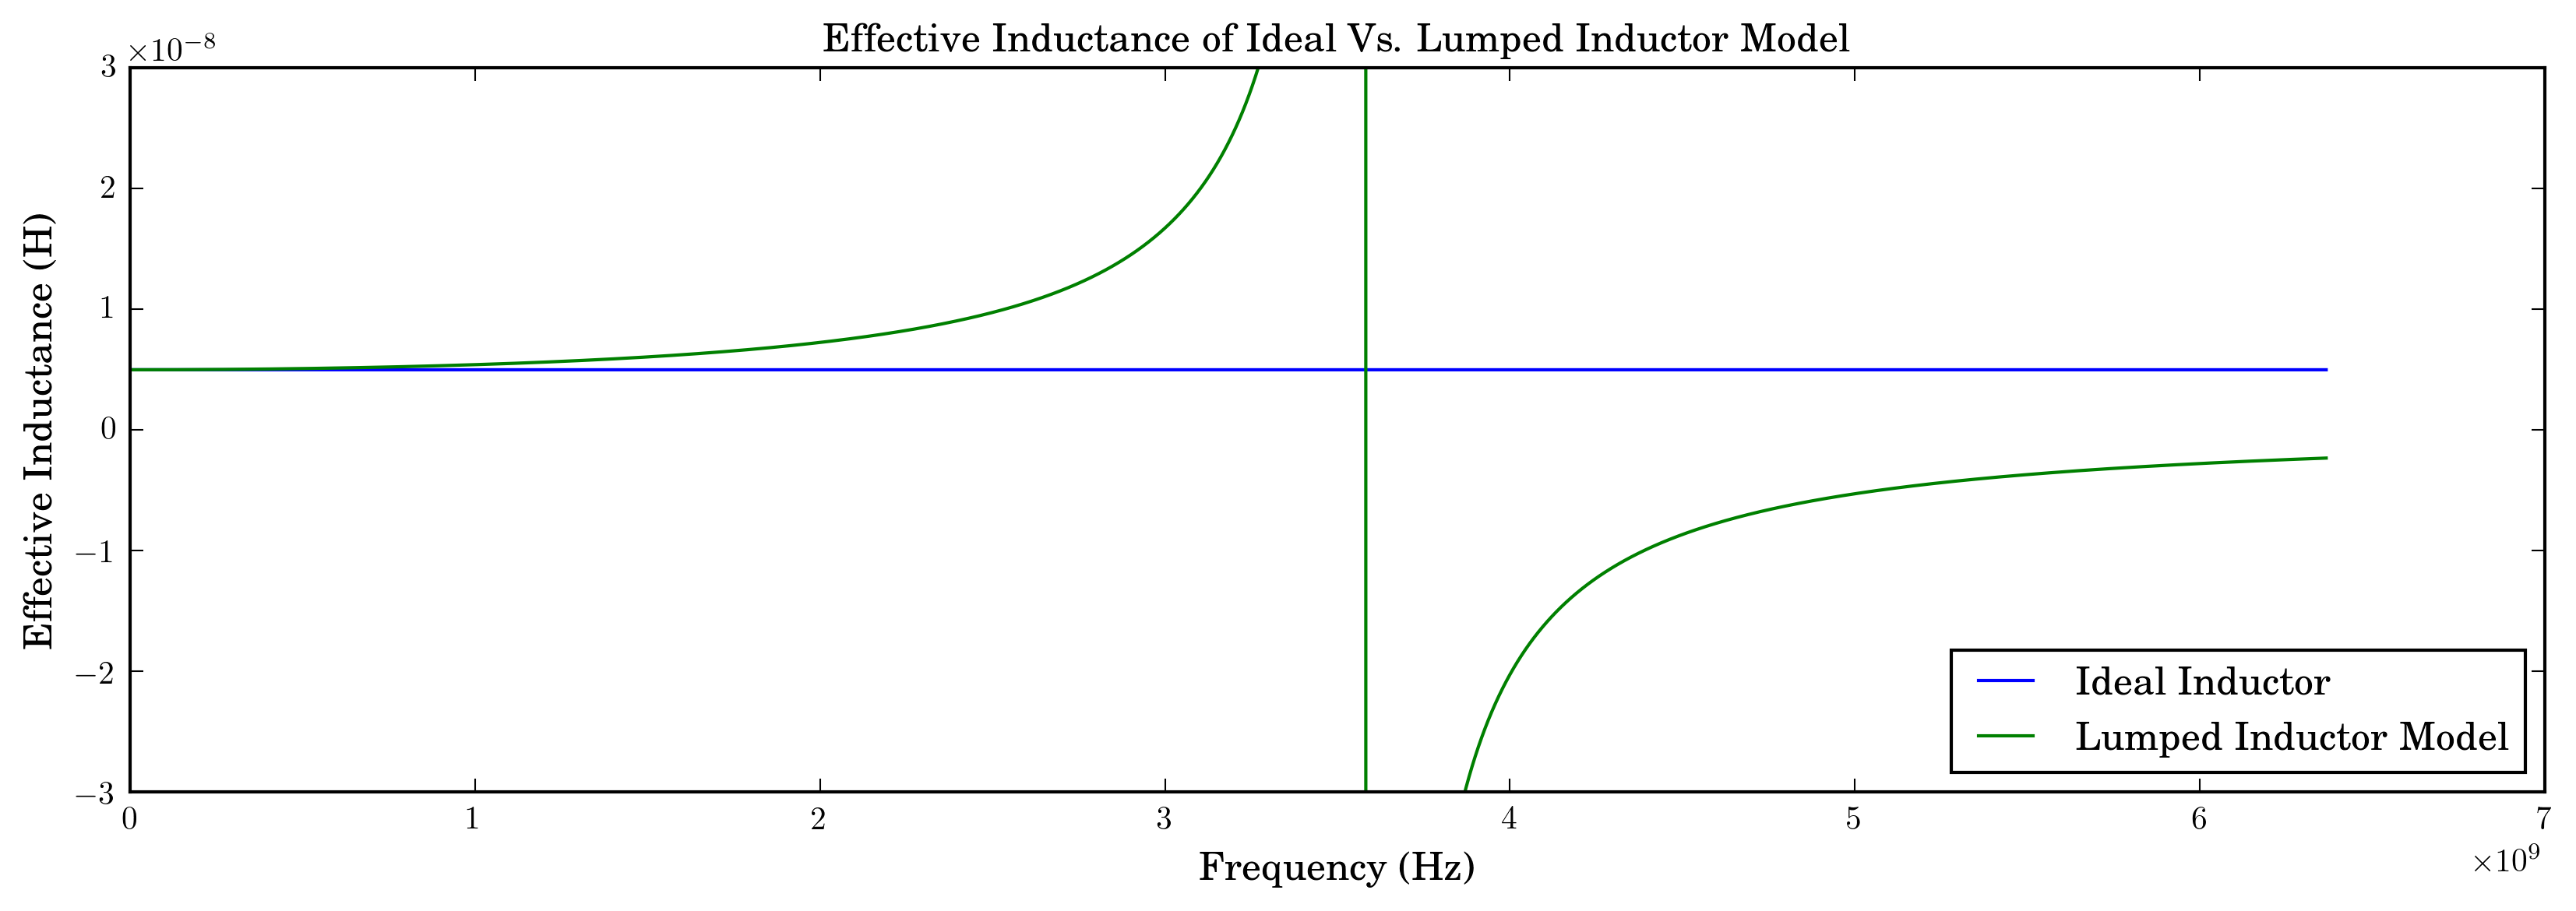
\includegraphics[width=\textwidth]{images/inductor_inductance.png}
\end{figure}

\subsubsection{Ideal Behavior}
The lumped inductor model has an inductance close to the ideal inductor up until around 3 Ghz. If we are more strict, it is only very close up to 1.5 Ghz.

\subsubsection{Self-Resonant Frequency}
From scanning the plot, the SRF should be around 3.5 Ghz. Calculating:

\begin{equation*}
	f_{resonance} \approx \frac{1}{2 \pi \sqrt{L C_{x}}} \rightarrow \frac{1}{2 \pi \sqrt{L (C_{x} + C_p)}} = 3.5 \text{ Ghz}
\end{equation*}

\subsubsection{Inductance Near SRF}
The effective inductance near SRF goes to 'infinity' (only damped by the resistor). After self-resonance, the inductor behaves like a capacitor with 'negative' inductance.

\subsubsection{Q-Factor}
\begin{equation*}
	Q = \frac{|X_L|}{R_x}
\end{equation*}
\begin{figure}[H]
	\centering 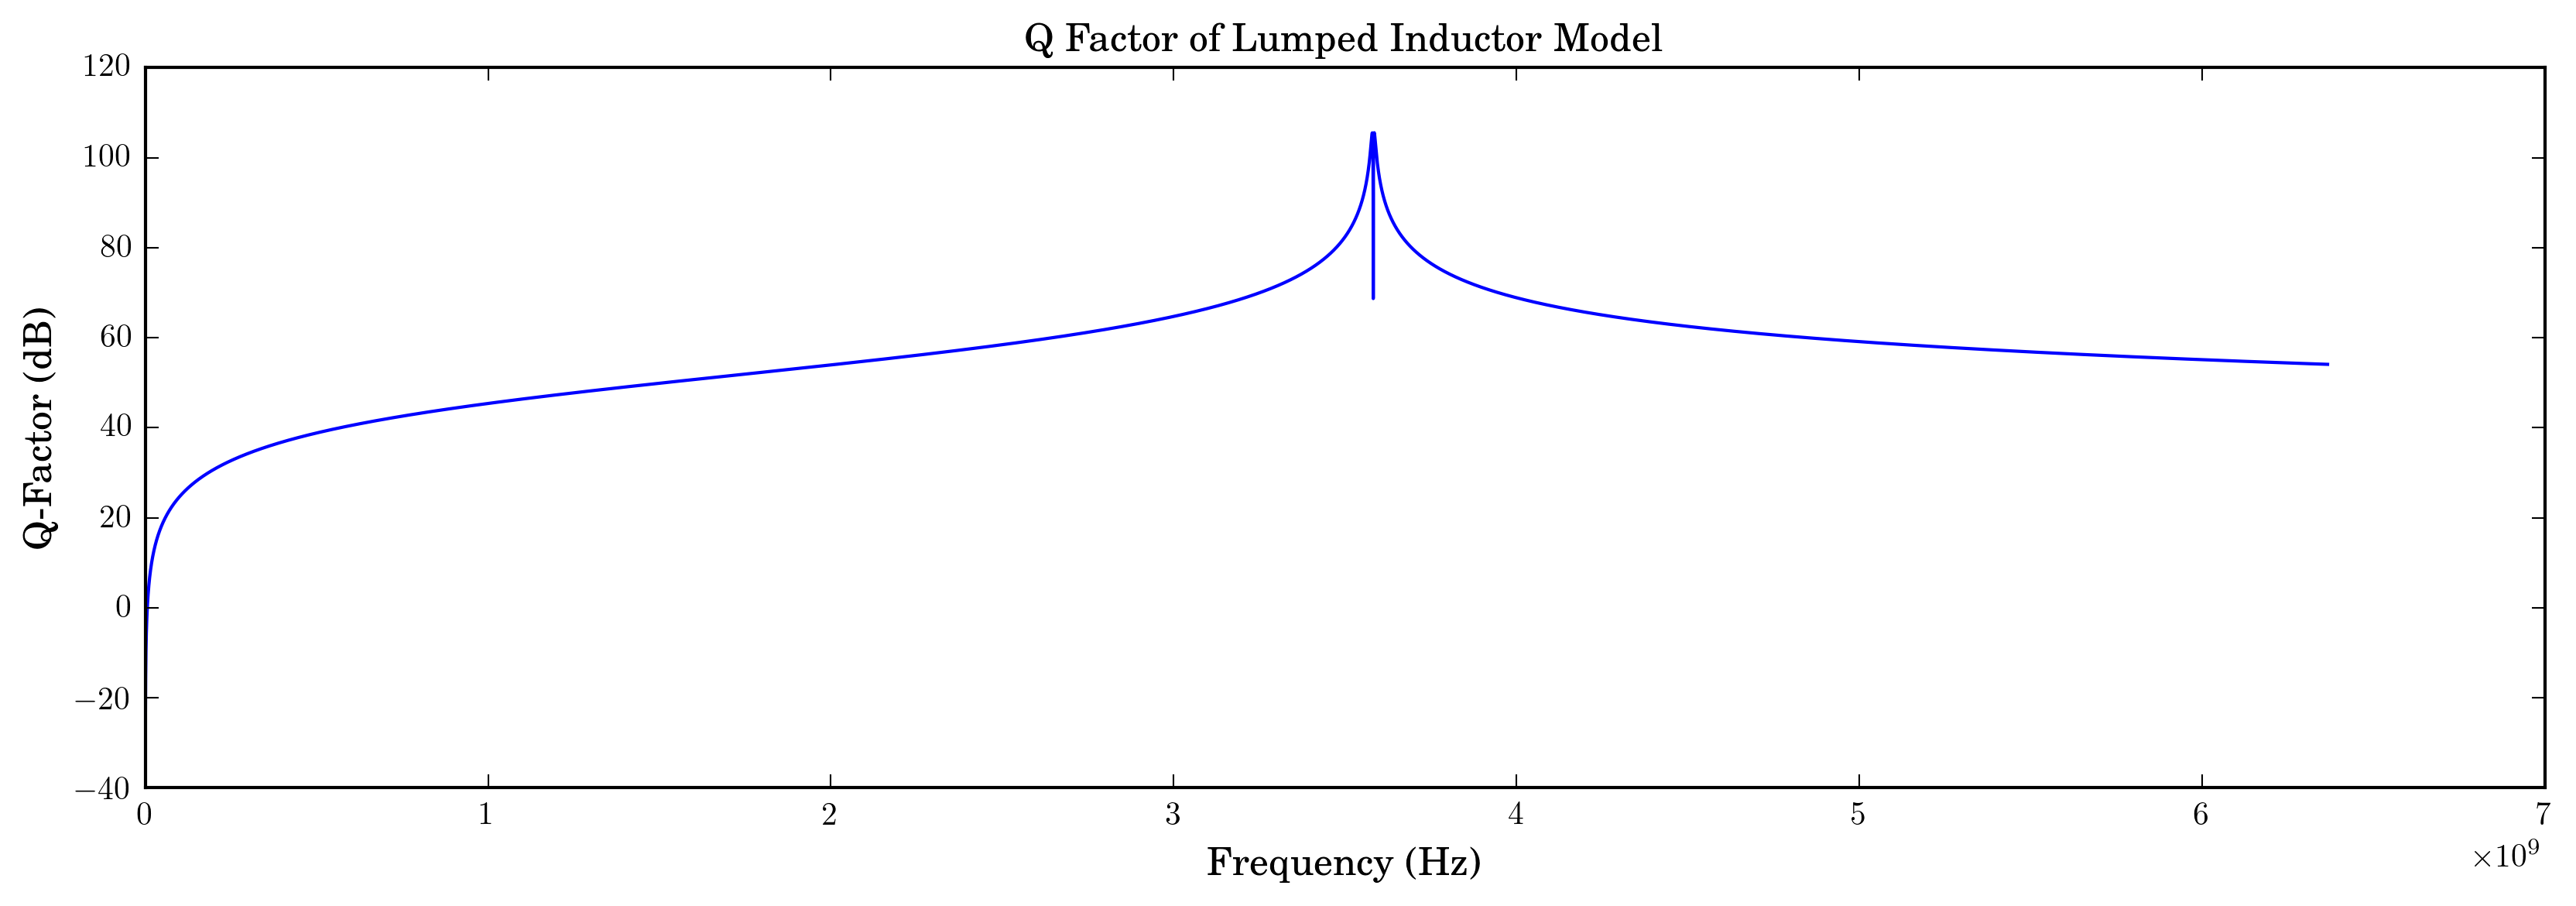
\includegraphics[width=\textwidth]{images/inductor_q.png}
\end{figure}

The inductor is very high Q over a very small range of a few Mhz.

\subsubsection{Smith Chart}
\begin{figure}[H]
	\centering 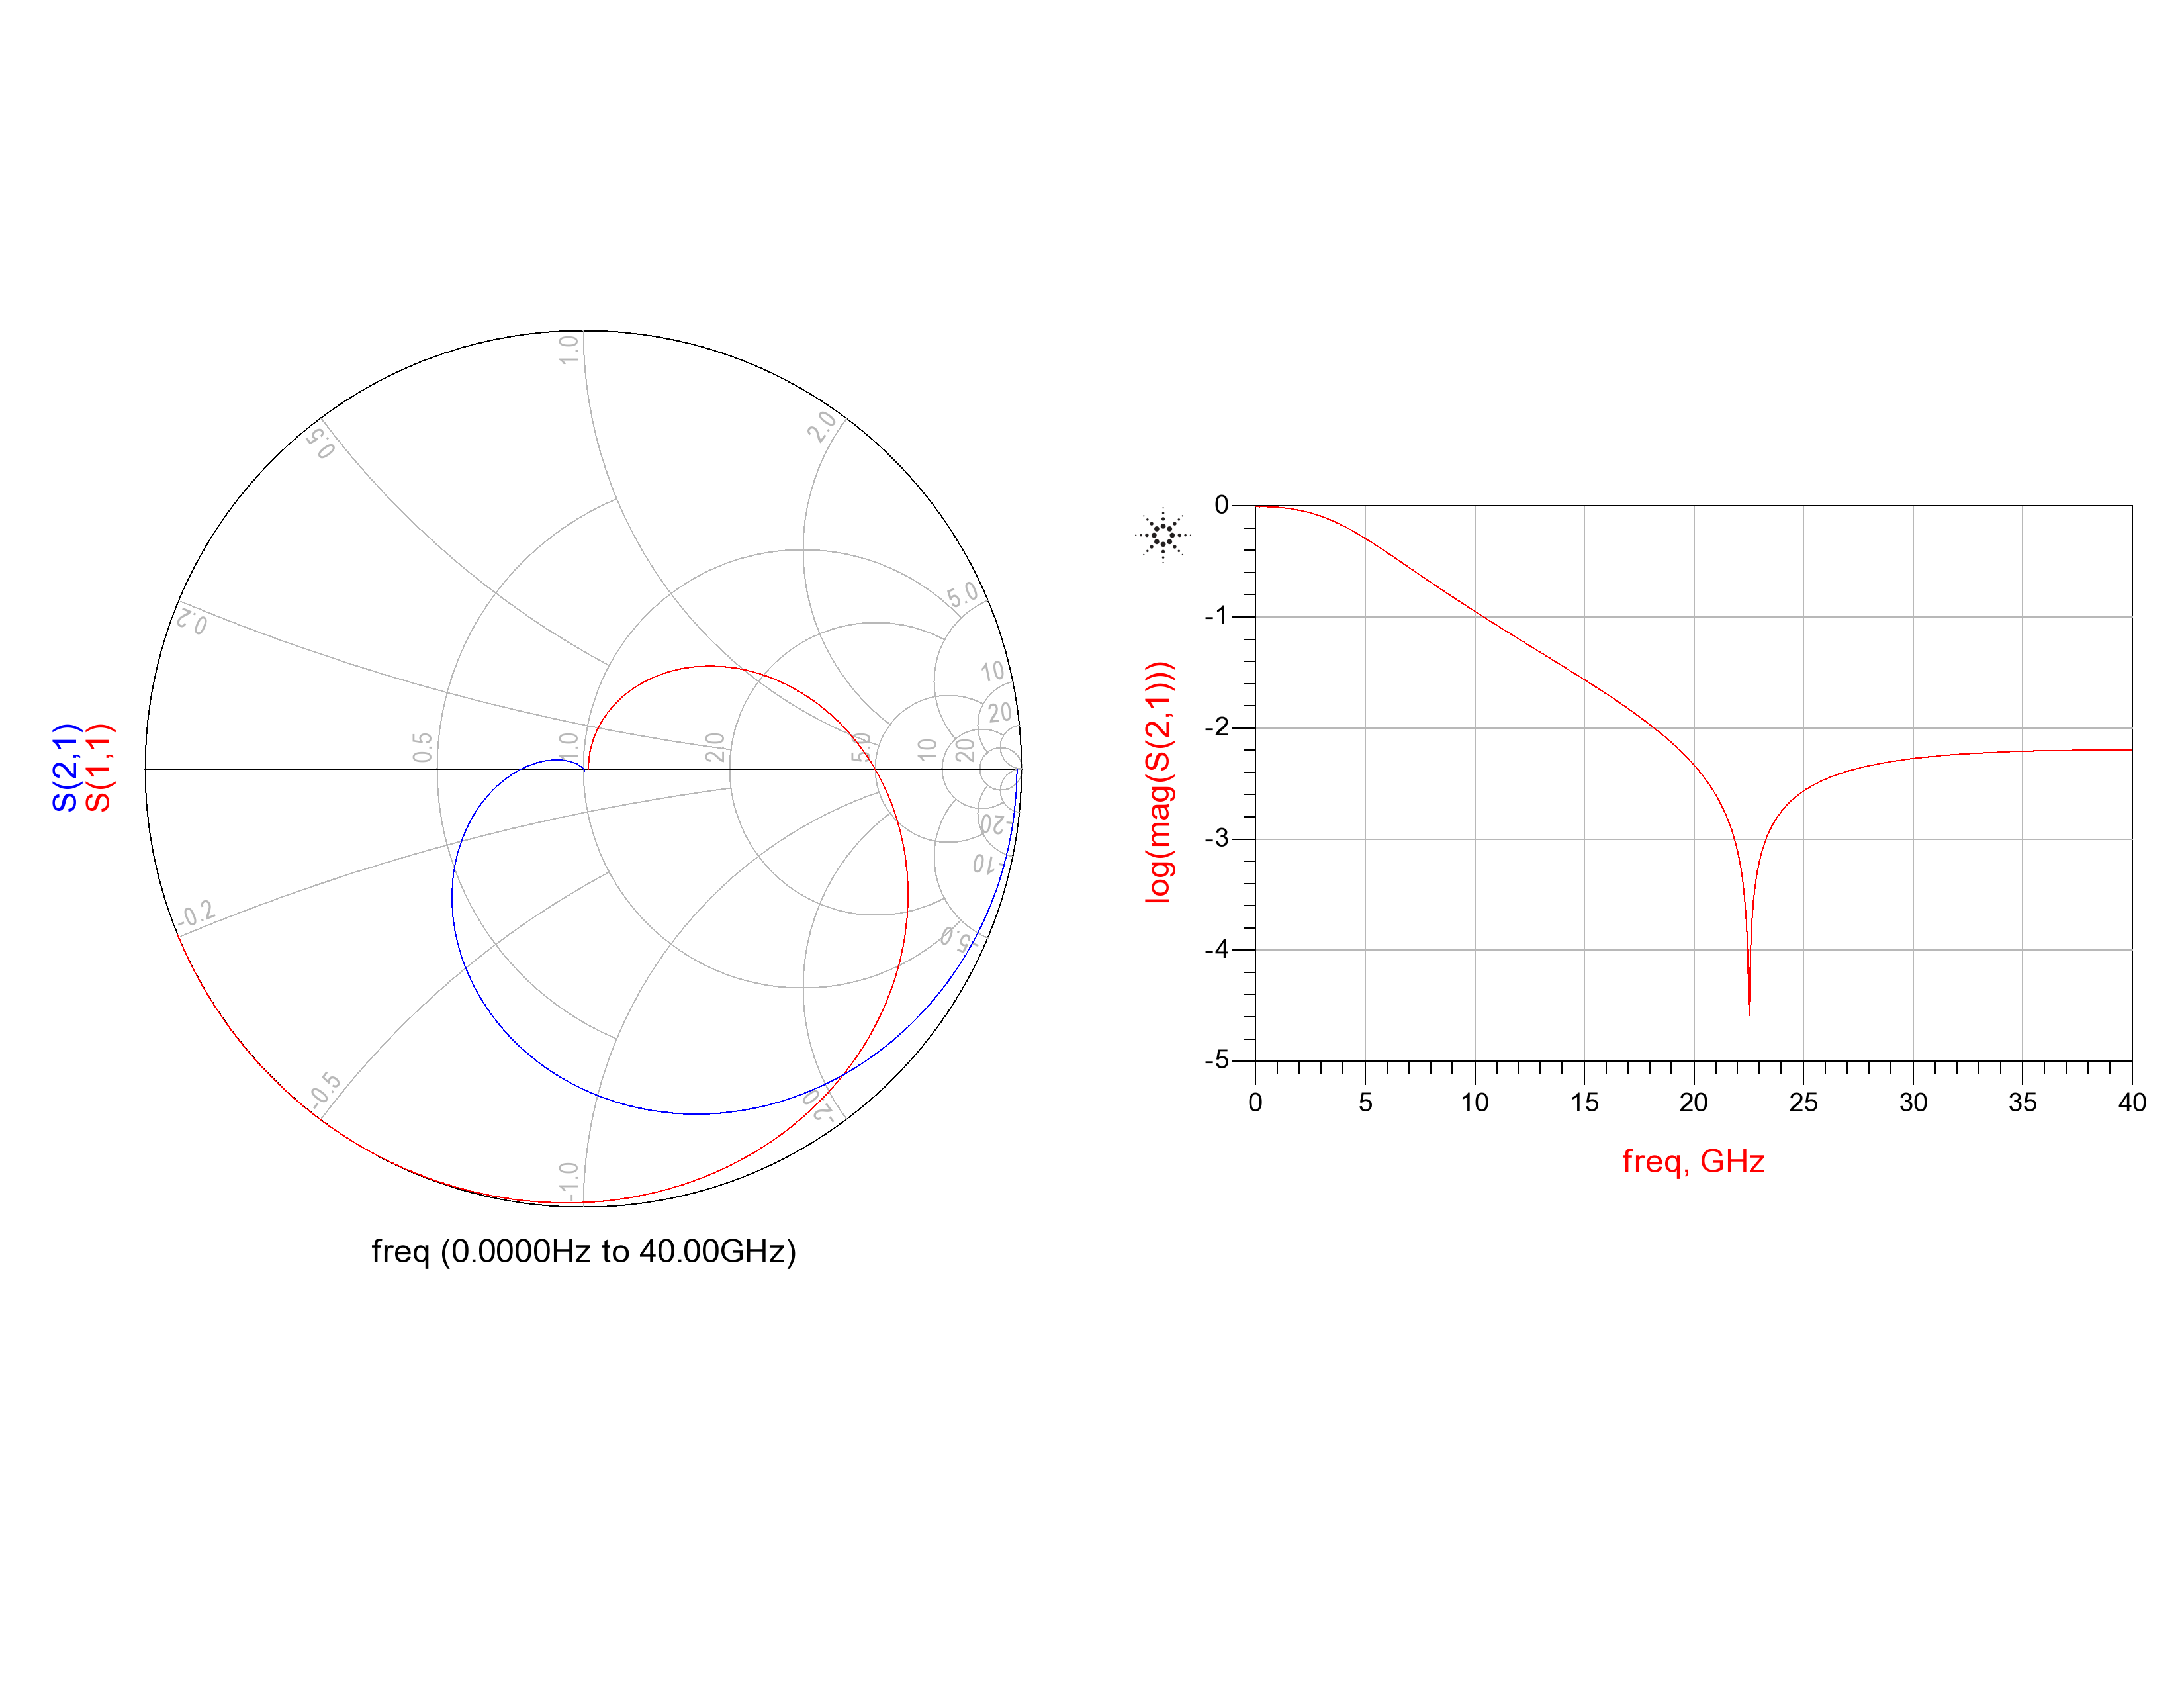
\includegraphics[width=\textwidth]{images/inductor_smith.png}
\end{figure}

\subsection{Distributed Inductor Model}
The component values are: $L = 5$ nH, $R_{x} = 1.15\Omega$, $C_{p} = 400$ fF, $C_{x} = 10$ fF.

We use a 5 part distributed inductor model with distributed $L_{w}$ and $C_{w}$ and $R_{w}$. The instructions given in the spec likely have typos, since it doesn't make sense to distribute $C_p$ along with the inductor (landing pads aren't distributed!).

\begin{figure}[H]
	\centering 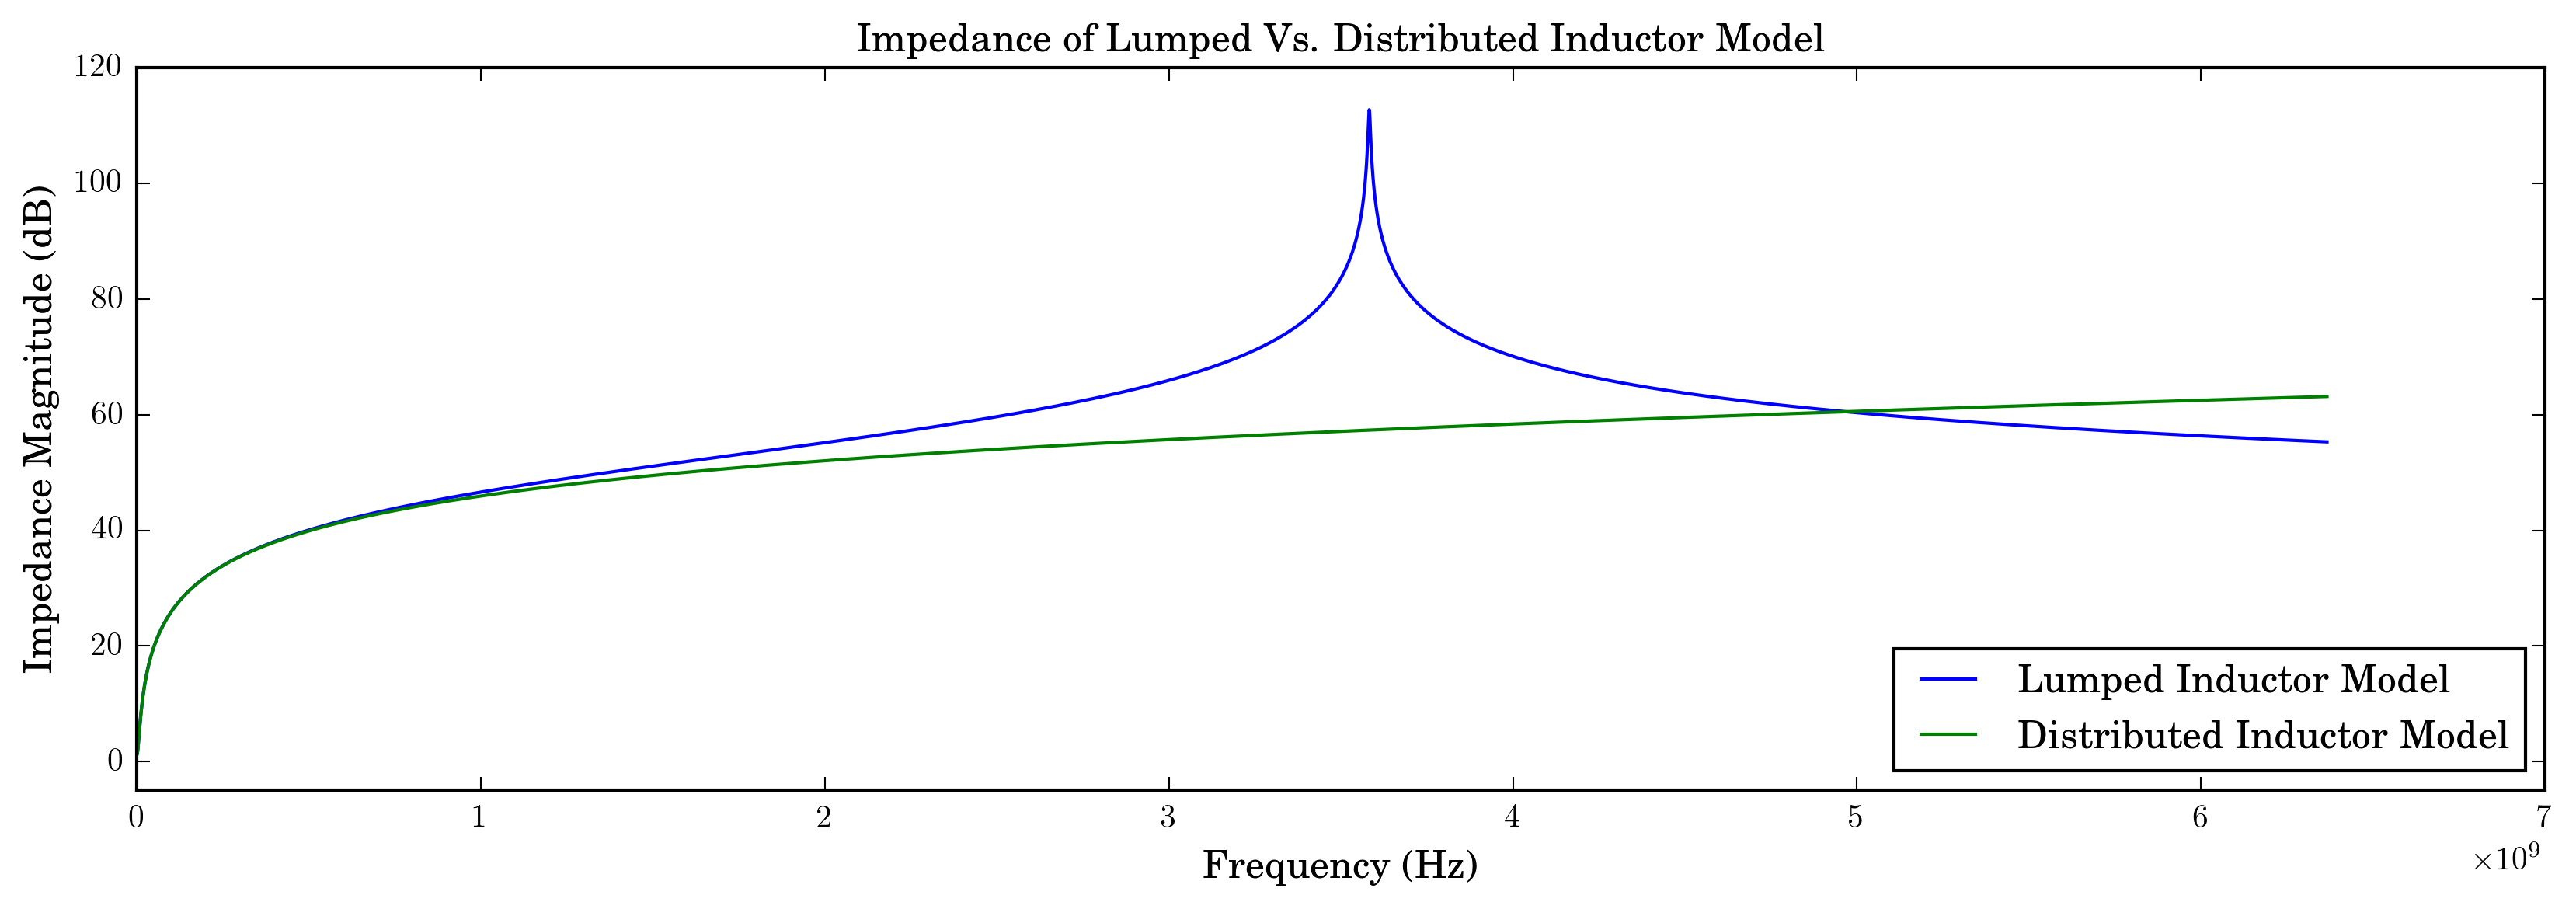
\includegraphics[width=\textwidth]{images/inductor_distr_impedance.png}
\end{figure}

The distributed inductor model doesn't resonate as expected due to each section resonating at the frequency 5x higher than the single lumped circuit. The distributed model will become more reflective of reality around $3.5 \cdot 5 = 17.5$ Ghz when resonance will take place within each winding and the impedance will again spike.

\subsection{Capacitor Analysis}
We consider a capacitor with component values: $C = 5$ pF, $R_x = 0.25\Omega$, $L_s = 0.75$ nH, $C_p = 20$ fF. We use the lumped capacitor model.

\begin{figure}[H]
	\centering 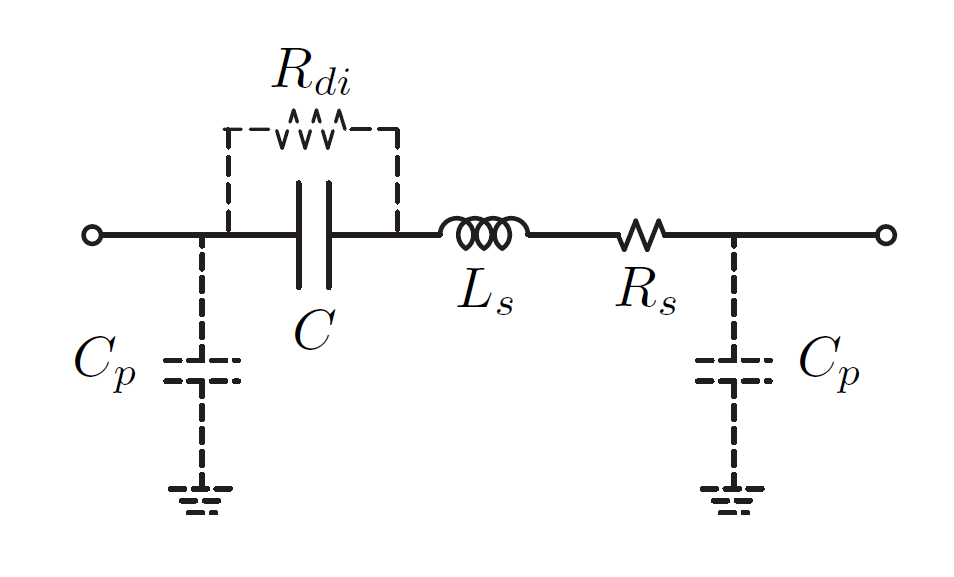
\includegraphics[width=\textwidth-8cm]{images/lumped_capacitor_model.png}
\end{figure}

\subsubsection{Impedance and Capacitance Plots}
\begin{figure}[H]
	\centering 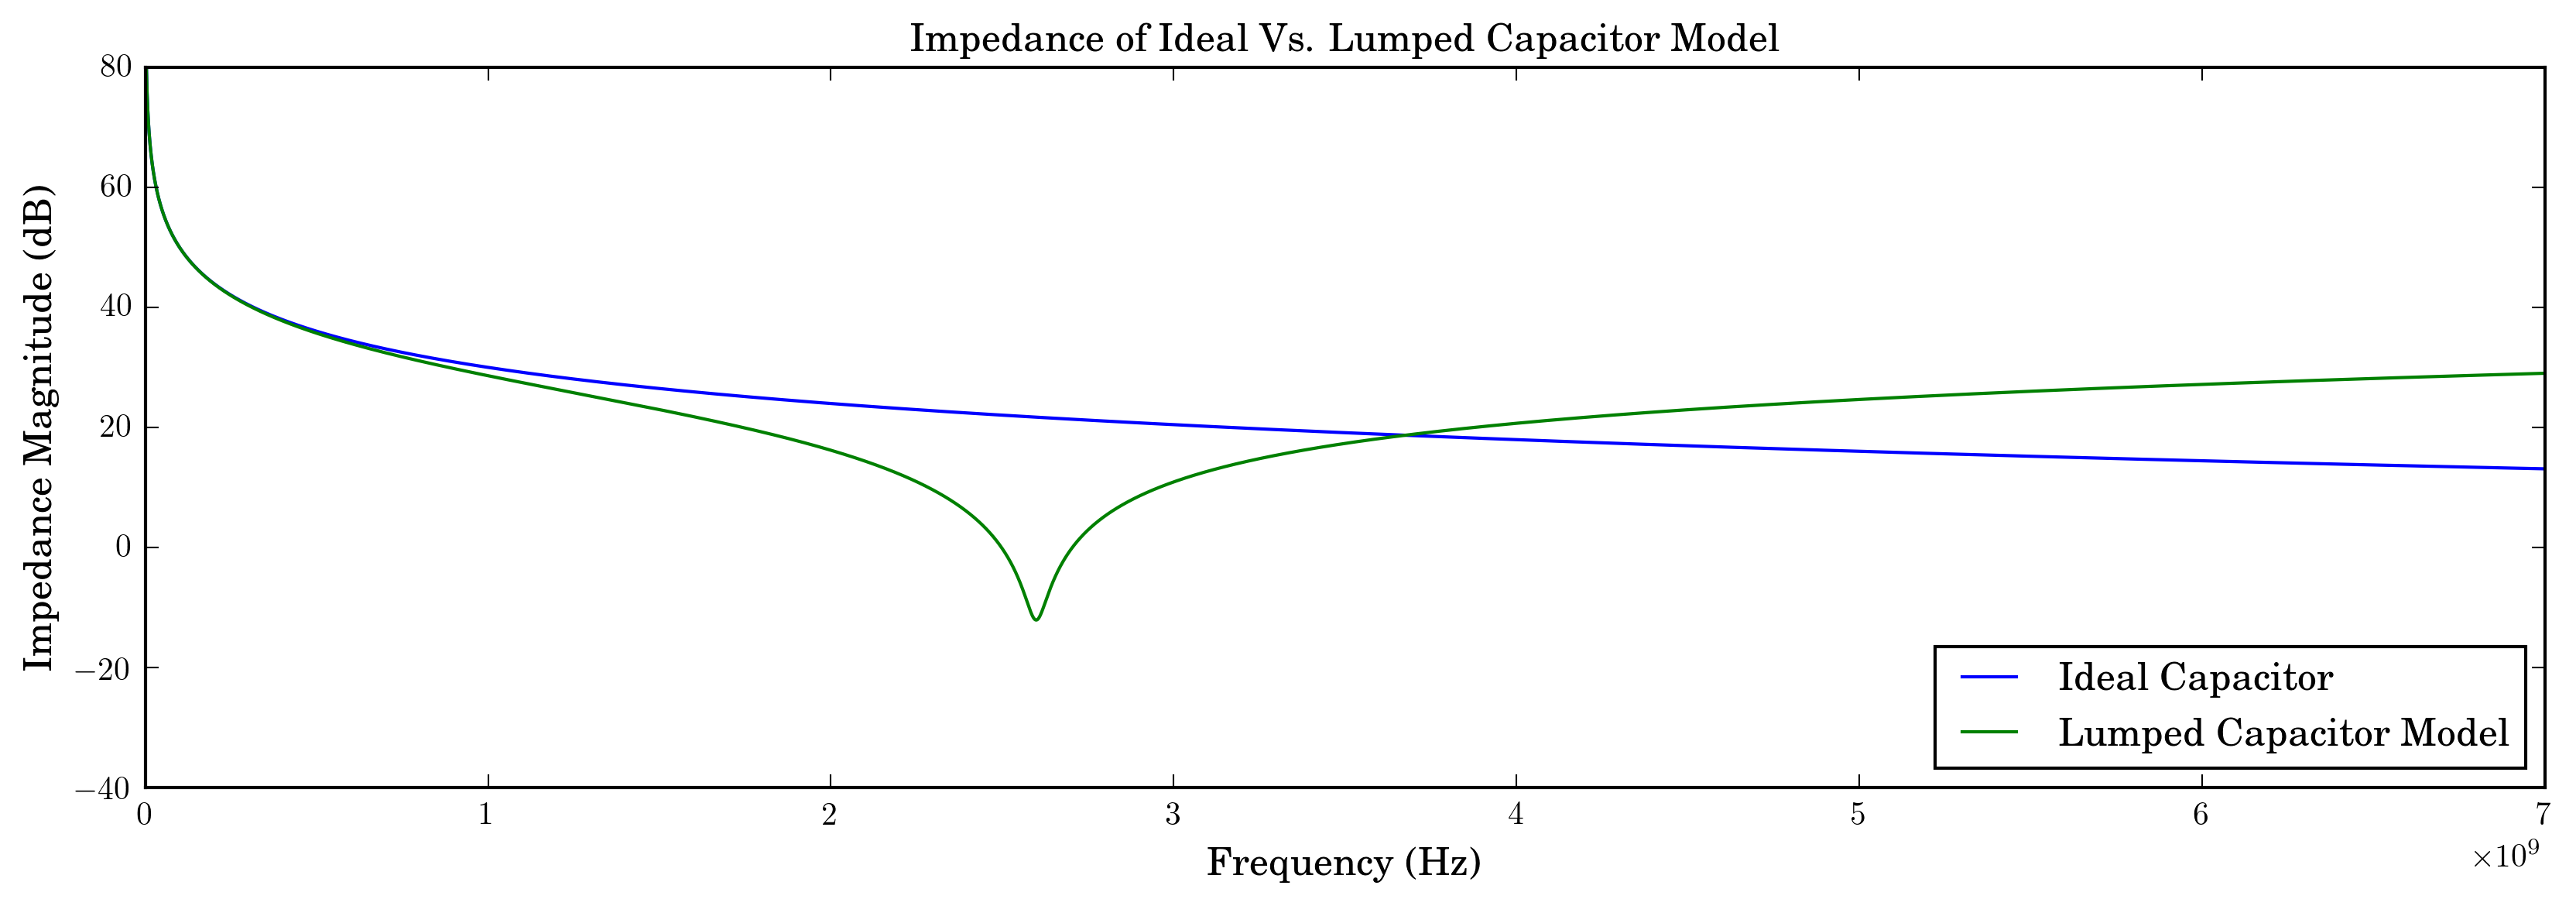
\includegraphics[width=\textwidth]{images/cap_impedance.png}
\end{figure}

\subsubsection{Effective Frequency Range}
\begin{figure}[H]
	\centering 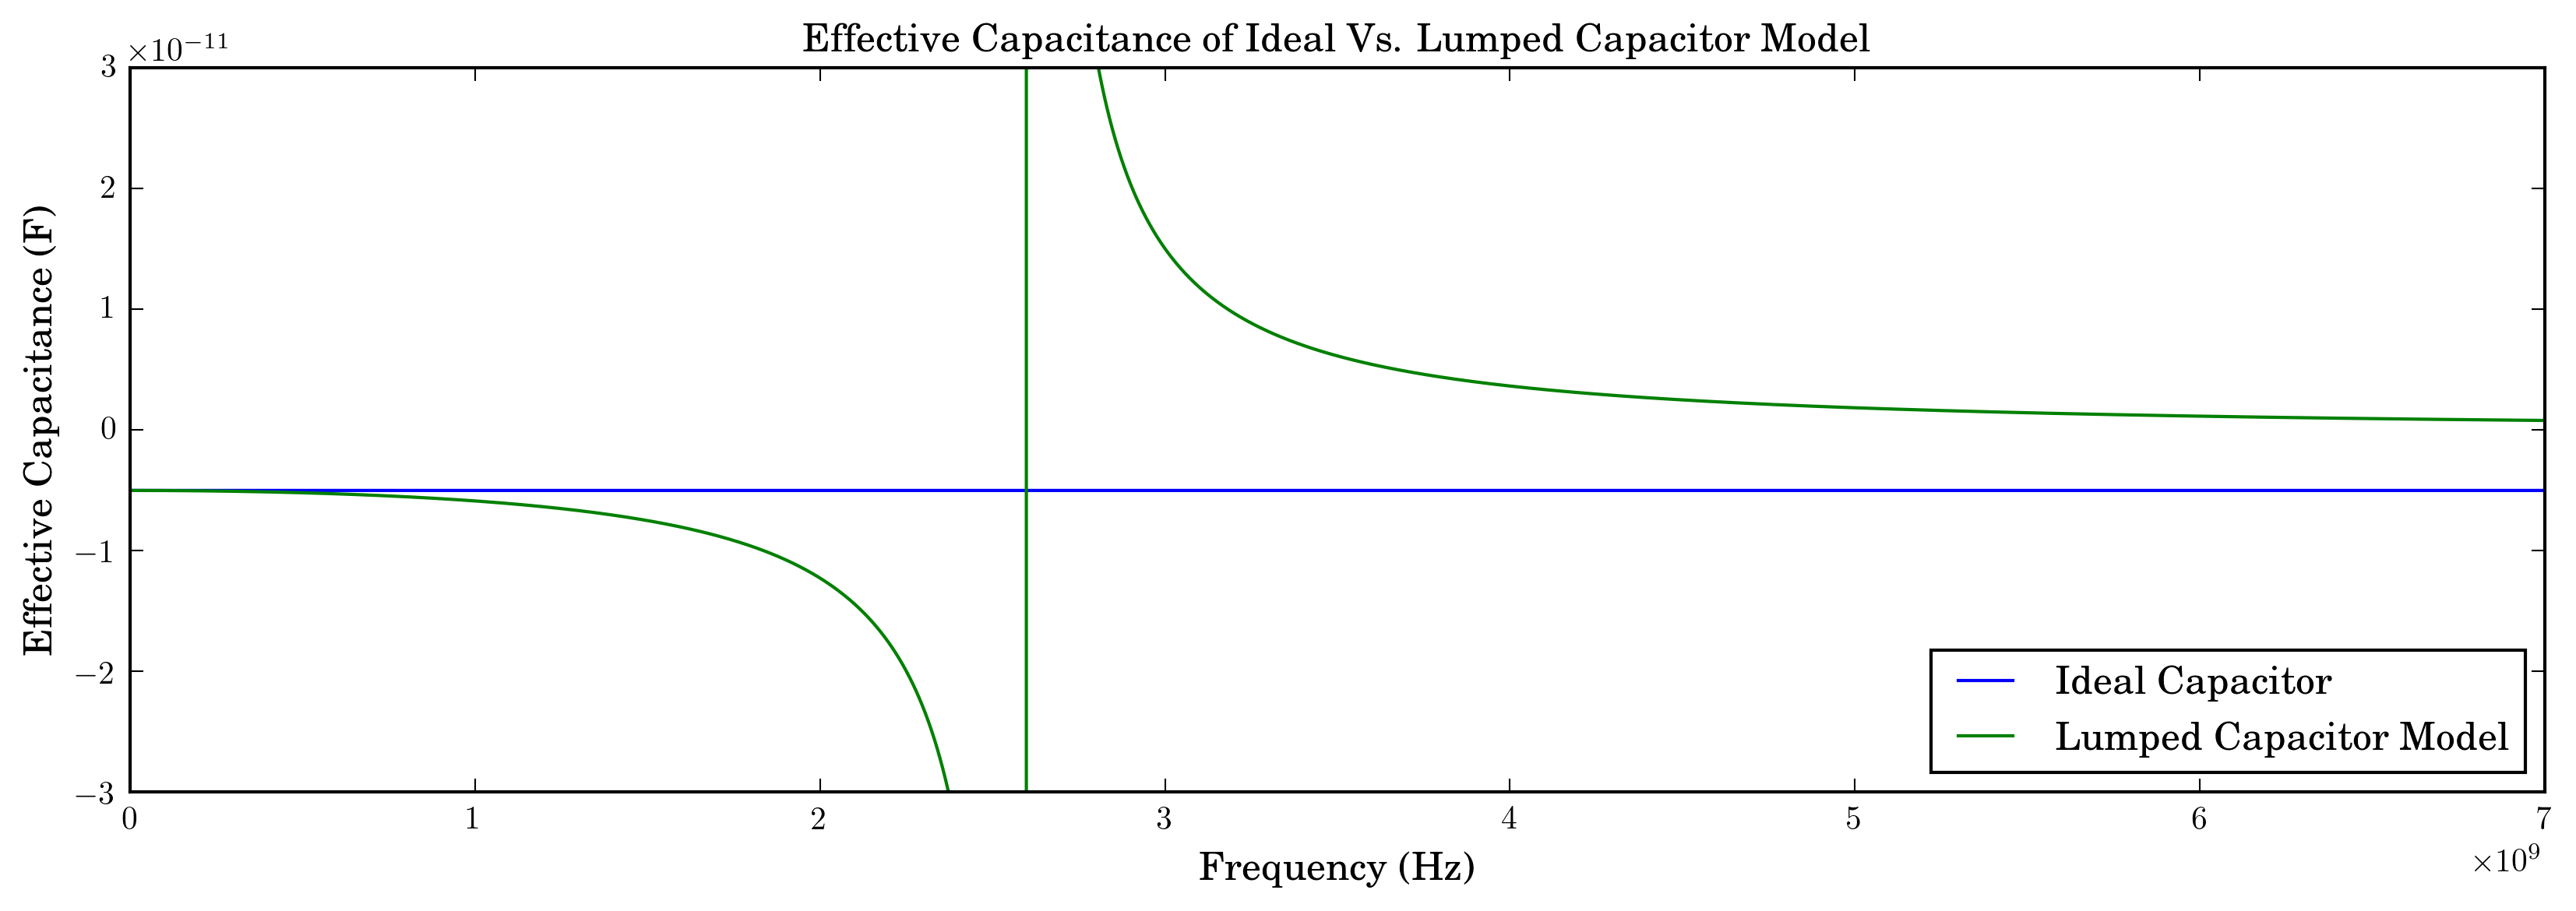
\includegraphics[width=\textwidth]{images/cap_capacitance.png}
\end{figure}

The capacitor is only close to the low frequency value below 1 Ghz. If you have a max deviation requirement of 10\%, then the non-ideal capacitor reaches 5.5 pF at 750 Mhz.

\subsubsection{Self-Resonance Frequency}
The SRF from the LC network only is 2.6 Ghz. The capacitance goes to (-) 'infinity' only limited by the series resistance as the circuit resonates.

\subsubsection{Q Factor}
\begin{figure}[H]
	\centering 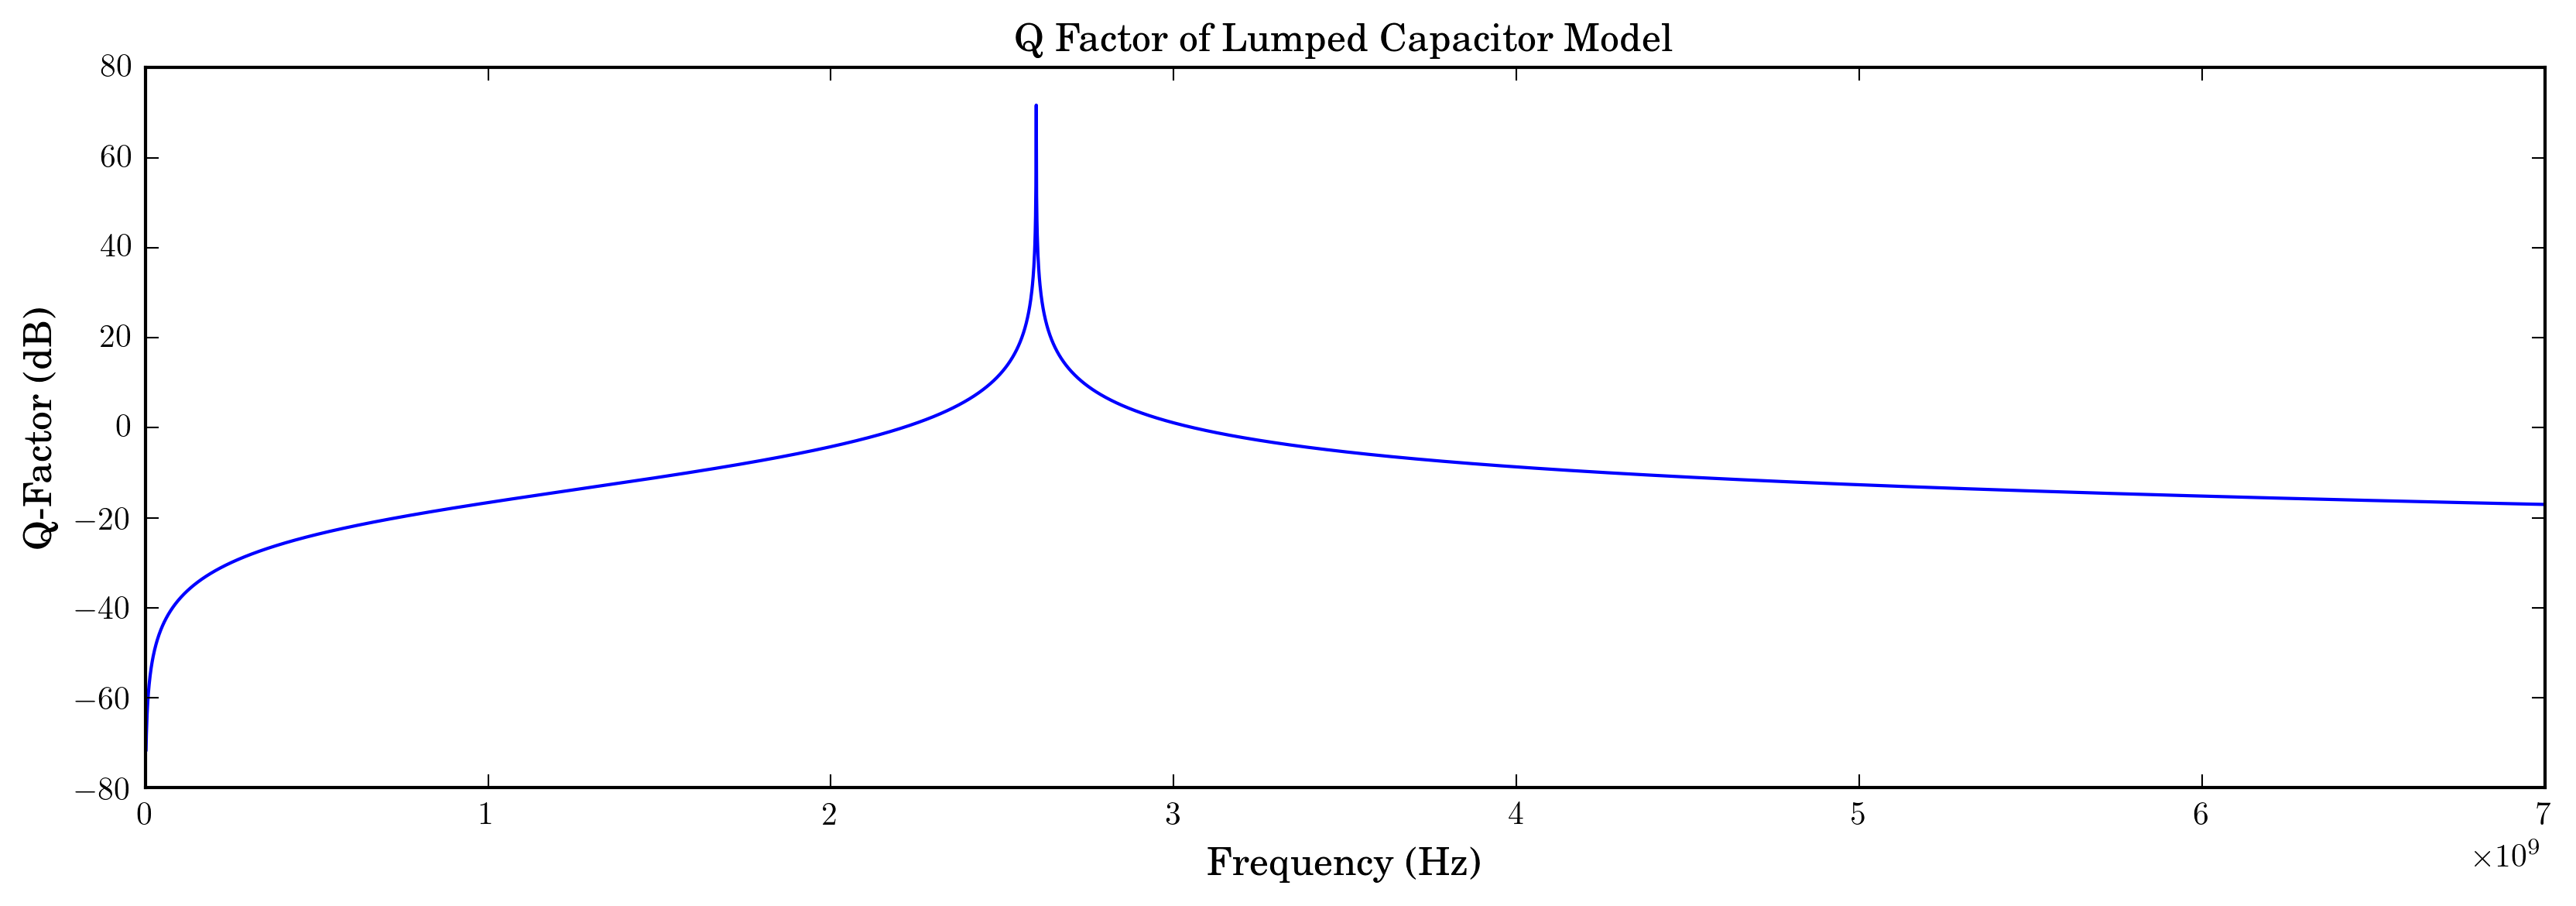
\includegraphics[width=\textwidth]{images/capacitor_q.png}
\end{figure}

\subsubsection{Smith Chart}
\begin{figure}[H]
	\centering 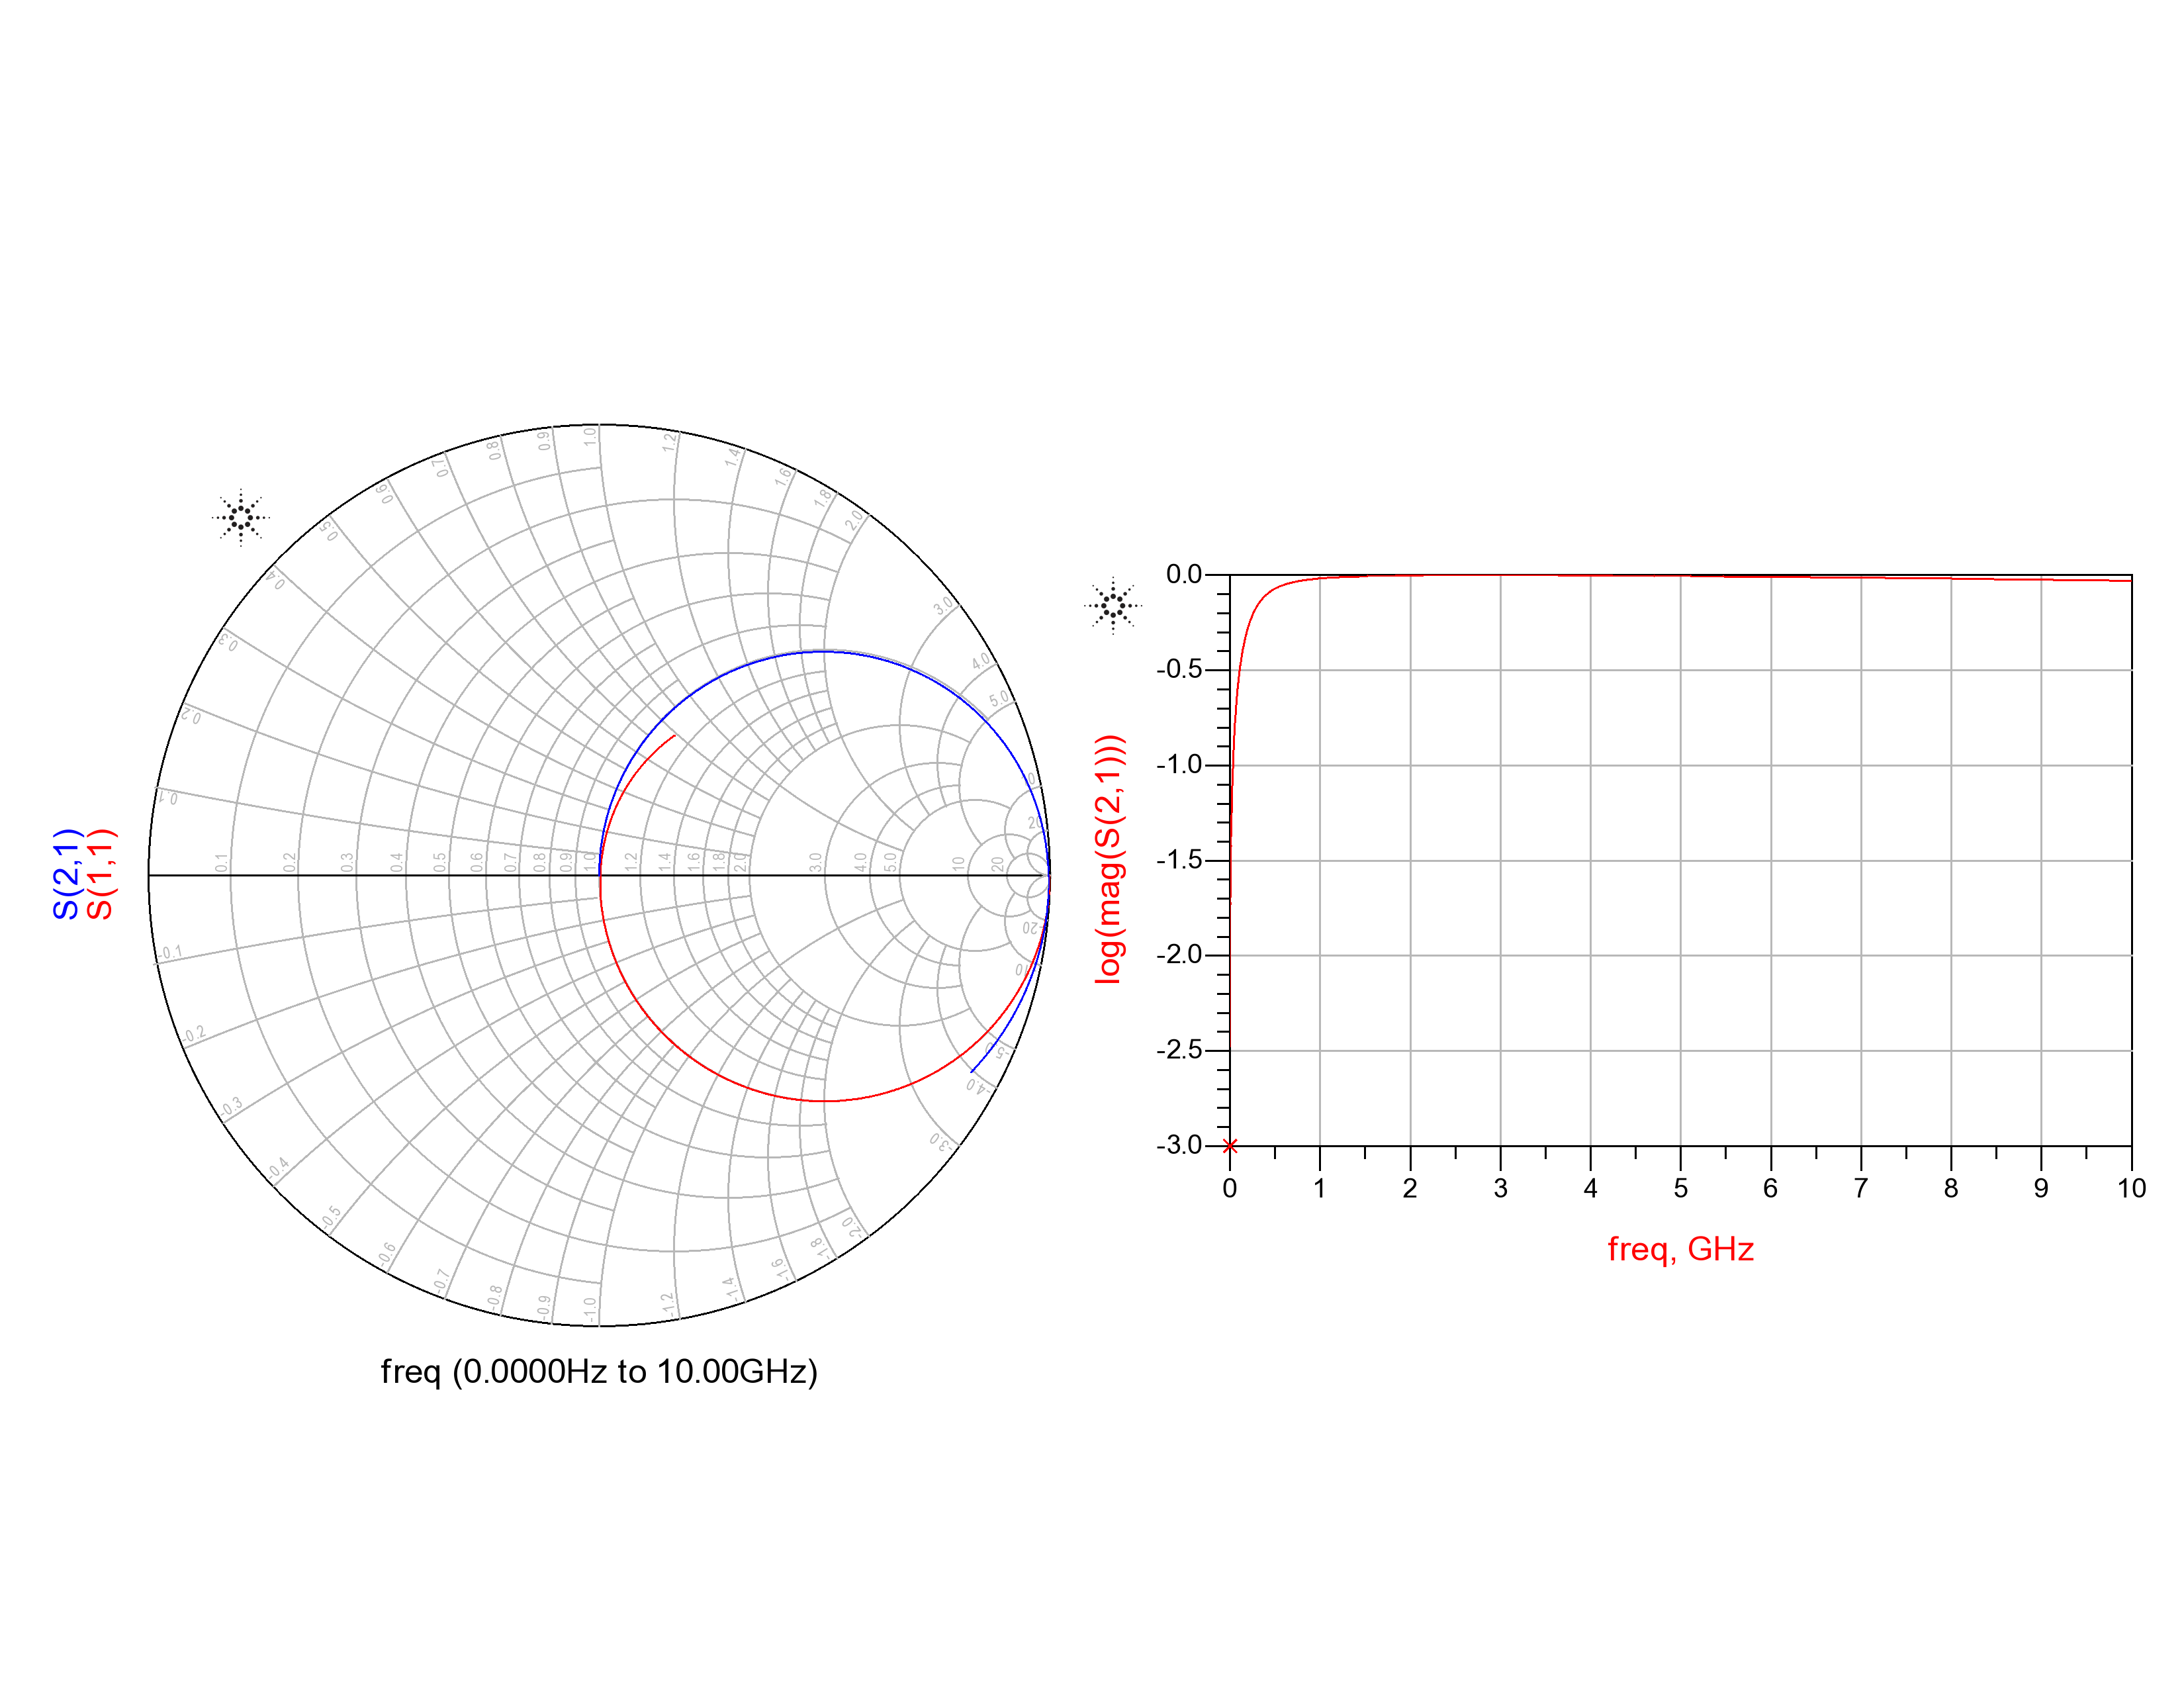
\includegraphics[width=\textwidth]{images/cap_smith.png}
\end{figure}

\end{document}
